\documentclass[12pt]{report}

\usepackage[a4paper,margin=2cm]{geometry}

%\evensidemargin = 0mm
%\oddsidemargin = 0mm
\topmargin = -30mm
\headheight = 0mm
\headsep = 20mm
\textheight = 240mm
%\textheight = 240mm
\textwidth = 170mm
%\leftmargin = 0mm
\parindent = 00mm
\baselineskip = 20mm
\lineskip = 1.0mm
\parskip = 1.5mm
\renewcommand{\baselinestretch}{1.5}
\usepackage{longtable}



\usepackage{cite}
\usepackage{float}
\usepackage{graphicx}
\usepackage{amsmath}
\usepackage{csquotes}
\usepackage{hyperref}
\usepackage[export]{adjustbox}
\usepackage{listings}
\usepackage{courier}
\usepackage{gensymb}

\lstset{basicstyle=\footnotesize\ttfamily,breaklines=true}
\lstset{frame=single}

\makeatletter

\newif\if@mainmatter \@mainmattertrue

\newcommand\frontmatter{%
	\cleardoublepage
	\@mainmatterfalse
	\pagenumbering{roman}}
\newcommand\mainmatter{%
	\cleardoublepage
	\@mainmattertrue
	\pagenumbering{arabic}}
\makeatother

\begin{document}

	%\chapter*{}

\thispagestyle{empty}
\vspace{1cm}

\begin{figure}[H]
	\centering
	
\includegraphics[width=0.25\linewidth]{unimelblogo.png}
	\label{unimelblogo}
\end{figure}

\vspace{1cm}

\begin{center}
	\Large{ \bf  Integrated Wireless Vital Signs Monitoring System for Specific Anaesthesia Parameters}
\end{center}

\vspace{1cm}

\begin{center}
	{\it  Submitted in partial fulfilment of the requirements of the Degree of }
\end{center}

\begin{center}
	{\bf   Master of Engineering (Electrical)}
\end{center}

\begin{center}
	{\it by }
\end{center}

\begin{center}
	{ \bf Jia Hui Ong (571319)}
\end{center}
\begin{center}
	{ \bf Jiayi Chen }
\end{center}
\begin{center}
	{ \bf William Kit Mun Ngeow (596301)}
\end{center}

\vspace{1cm}

\begin{center}
	{\it Department of Electrical and Electronic Engineering }  \\
	{ \it  The University of Melbourne   }  \\
	{ \it  Victoria 3010   }   \\
	{ \it  AUSTRALIA   }
\end{center}

\vspace{1cm}

\begin{center}
	{\bf  October 2016 }
\end{center}


	\frontmatter
	\chapter*{Acknowledgements}

This Capstone Project and its supplementary achievements could only have been accomplished through the support of a number of individuals, to whom we would like to extend our thanks. \\

It is our desire to express our heartfelt thanks and gratitude to our supervisor Dr. Palaniswami for his unparalleled guidance and direction in our project. He has been the most influential person in motivating us to do beyond what we thought we could. \\

We would like to extend our sincere appreciation to Dr. Colin Iatrou and Dr. Terrence Caelli, without whom this project would not be possible. They have provided unprecendented insight into the field of medical anaesthesia and wireless systems, which has laid the foundation for our pursuit. \\

We would also like to thank Rajesh Ranjan, who has been ever willing to assist us when we were in need, both academically and practically. \\

Lastly we would like to thank our friends and family, the unsung heroes and heroines who believed in and supported us unconditionally in every possible way. \\

	
\chapter*{Symbols and  Acronyms}
  

\vspace{1cm}

In this paper, we  will  use the  following  acronyms:
\begin{align*}
\mbox{WVSMS} & =  \mbox{Wireless Vital Signs Monitoring System}    \\
\mbox{ECG} & =  \mbox{Electrocardiography}     \\
\mbox{EEG} & =  \mbox{Electroencephalography}     \\
\mbox{PPG} & =  \mbox{Photoplethysmography}    \\
\mbox{LED} & =  \mbox{Light Emitting Diode} \\
\mbox{OS} & =  \mbox{Operating System}	\\
\mbox{VNC} & =  \mbox{Virtual Network Computing}  \\
\mbox{CPU} & =  \mbox{Central Processing Unit}  \\
\mbox{LAN} & =  \mbox{Local Area Network}  \\
\mbox{HDMI} & =  \mbox{High-Definition Multimedia Interface}  \\
\mbox{SD} & =  \mbox{Secure Digital (Non-volatile memory card format)}  \\
\mbox{USB} & =  \mbox{Universal Serial Bus}  \\
\mbox{GPIO} & =  \mbox{General-Purpose Input/Output}  \\
\mbox{ARM} & =  \mbox{Advanced RISC Machines (Processor)}  \\
\mbox{WiFi} & =  \mbox{Wireless LAN (WLAN)}  \\
\mbox{IoT} & =  \mbox{Internet of Things}  \\
\mbox{IC} & =  \mbox{Integrated Circuit} \\
\mbox{PCB} & =  \mbox{Printed Circuit Board}  \\
\end{align*}


\begin{align*}
\mbox{NTC} & =  \mbox{Negative Temperature Coefficient (Thermistor)}  \\ 
\mbox{PSO} & =  \mbox{Phase Shift Oscillator}  
\end{align*}

	
\chapter*{Abstract}

This report documents the design and development process of a wireless vital signs monitoring system by Master of Engineering (Electrical) students at the University of Melbourne. The project aims to assemble a completely wireless system with attached sensors which is as reliable and accurate as current conventional monitoring systems.  

In modern surgery, there is an ever increasing number of devices attached to a patient in the surgery room. The presence of wire bundles introduces implicit hazards which could possibly harm the patient or the surgeons. To mitigate and circumvent this issue, the number of wires could be reduced through the implementation of wireless vital signs monitoring systems in operating theatres.  

The wireless vital signs monitoring system consists of a main operating terminal and connected sensors. The anaesthetic parameters chosen for observation are electrocardiography (ECG), electroencephalography (EEG), photoplethysmography (PPG), blood temperature, and blood pressure. 

The terminal is designed for data processing, data transmission, and data visualisation. To do this, the Raspberry Pi 3 Model B was chosen due to its desirable properties as a miniaturised computer and fulfills the platform requirements of the project. It runs applications on an ARM processor loaded with a Linux-based Raspbian Jessie operating system. In terms of wireless transmission, it is fully capable of WiFi transmission and establishing a VNC server for secured external access. 

The sensors are designed individually with analog inputs and these signals are fed into analog-to-digital converters. The converted digital signals are then processed by applications on the terminal to be visualised and then transmitted wirelessly to another terminal for displaying the output. 

Both the terminal and sensors have been tested. The terminal has successfully collected signals from different sensors and transmitted them across to a second platform to be displayed. Additionally, the sensors circuit testing shows multiple sensors to be fully working and accurate. 


	
	\tableofcontents
	\listoffigures
	\listoftables
	
	
	\mainmatter
	\chapter{Introduction and Background}

\section{The Spaghetti Syndrome and its Implications - the need for a Wireless Vital Signs Monitoring System}

Modern surgeries are challenging working environments involving a combination of complex devices, computers and humans working under stressful and time critical conditions. However, to date there are far too many wired devices communication between machines, monitoring patient physiological conditions and still requiring considerable attention by experts for monitoring and decision making.

In an era where surgery is ubiquitous, an ever increasing number of devices are attached to critically ill patients, multiplying the number of wires and tubes connected to the patient which results in a net resembling a plate of spaghetti; hence, the coinage of the term the Spaghetti Syndrome \cite{imhoff2004spaghetti}. This conundrum has been present in the context of critical care, anaesthesia, and operating theatres for almost three decades with the advent of new technological advances in medicine \cite{cesarano1979spaghetti}. This issue clearly illustrates the need for a system which is not physically connected to avoid possible harm and injury to both the surgeons and patients in the operating theatre. 

The presence of wires in the surgery room introduces the possibility of increased surgery duration due to tripping hazards. More severe trips could lead to further surgical complications, due to wire disconnections which results in inaccurate readings of vital signs. Consequently, a possible overdose or underdose of anaesthetic agents could follow, leading to patient injury, and in the worst case scenario, the demise of the patient. Indirectly, wires in the operating theatre increase the rate of mortality during surgeries. 

One possible course of action to rectify this problem is to remove cables connected to patients by replacing the medium of transmission from a wire to electromagnetic waves. In recent years, multiple research projects have been carried out with the aim to embed vital sign sensors with wireless technology to separate patients from cables \cite{rosenthal2003new}.  

Nevertheless, most advances in this area of wireless device development is limited to the context of medical centres and not operating theatres.  

\section{Benefits of a Wireless Implementation}

Having a wireless version of current vital signs monitoring systems will bring additional benefits to 


Ease of use - convenience
Less risk of injury
Faster surgery - smaller delay due to obstruction from wires
Safer
Better working environment for doctors

\section{Overview of the Project}

This  paper will  consider the  process and challenges of  developing a fully integrated wireless vital signs monitoring system for vital signs specifically for anaesthetic parameters such as electrocardiography (ECG), photoplethysmography (PPG), electroencephalography (EEG), blood pressure, and blood temperature. The  front end of the project encompasses the collection and processing of raw data from different sensors including the visualisation and presentation of vital signs information,  according  to some specified performance criterion. The back end of the project involves the wireless transmission and reception of the processed information to a fixed output display and possibly, a secure database. 

The aim of this project is to make as many patient monitoring, measuring devices as fully wireless so enabling more freedom of movement for both patients, nurses, and medical staff. What makes this first task challenging is that the wireless network (WA) system must be safe, secure and as reliable as current wired systems. Once completed, we envisage a new program in the development of pervasive wireless network resources for anesthetists and surgical practice in general. In these cases being hands-free, being able to access information, direct activities by simple movement, gestures adds to more efficient and clean surgical practice. \\

The project involves two parts: 

\begin{enumerate}
	\item programming hardware nodes to collect wireless sensor data using Android, and 
	
	\item software application development to visualize the data in real-time. The project also involves estimating missing data and inferring suitable information to medical professionals. The project requires developing a mobile app and also a data analysis platform.
\end{enumerate}


\section{Anaesthetic Parameters for Patient Monitoring}

Countless operations are conducted on a daily basis which requires patients to be under general anaesthesia. To ensure the patient's optimal safety when under anaesthesia, it is necessary to consistently monitor certain parameters to ensure that they remain within a specified range which is considered to be safe or normal. Based on Atlee's Complications in Anesthesia \cite{atlee2006complications}, monitoring of anaesthetic admisnistration reduces the probability of anaesthetic overdose or underdose. 

Complications associated with an improper dosage of anaesthesia could arise such as coma, brain damage, nerve damage, or possibly death, if real-time observations of vital signs are not conducted. The risk of such issues occuring during surgery could be reduced significantly if a feedback system were implemented for the amount of anaesthetics administered to the patient. Such parameters have been stipulated by ANZCA. 

\subsection{Theory of Electrocardiography}

The electrocardiogram (ECG) refers to the recording of the "differences in electrical potential generated by the heart" using electrodes which are placed on the surface of the skin \cite{noble1990electrocardiography}. Both the action potentials generated by individual cells and sequence of activation affect the signal registered during electrocardiography \cite{noble1990electrocardiography}. Other factors which alter the final signal include "the position of the heart within the body, the nature of the intervening tissue, and the distance to the recording electrode" \cite{noble1990electrocardiography}. Despite the many factors which can possibly contribute a change to the electrocardiogram, it is still possible to deduce with high accuracy the state of the heart from the surface ECG due to "the careful correlation of electrocardiographic patterns with observed anatomic, pathologic, and physiologic data" \cite{noble1990electrocardiography}. 


\begin{figure}[H]
	\centering
	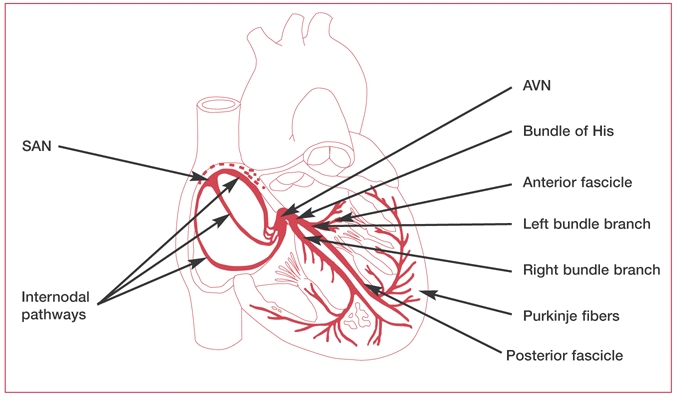
\includegraphics[width=0.7\linewidth]{ch3f3.jpg}
	\caption{The Cardiac Depolarization Route. AVN: Atrioventricular Node; SAN: Sinoatrial Node. \cite{hall2015guyton}}
	\label{cardiacdepolarization}
\end{figure}

\begin{figure}[H]
	\centering
	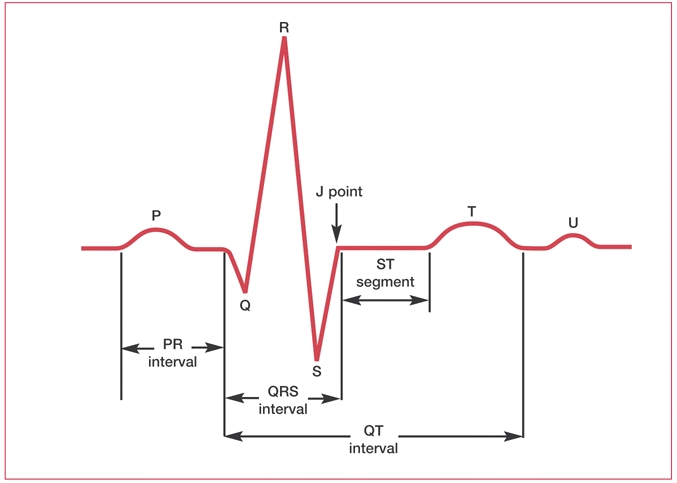
\includegraphics[width=0.7\linewidth]{ch3f4.jpg}
	\caption{The Basic Pattern of Electrical Activity across the Heart \cite{ashley2004conquering}}
	\label{ecgpattern}
\end{figure}

Figure \ref{ecgpattern} shows a graphical representation of a typical electrocardiograph trace of the electrical signals from the heart. 

The basic ECG pattern is correlated as follows: 

\begin{itemize}
	\item "Electrical activity towards a lead causes an upward deflection" \cite{ashley2004conquering}
	\item "Electrical activity away from a lead causes a downward deflection" \cite{ashley2004conquering} 
	\item "Depolarization and repolarization deflections occur in opposite directions" \cite{ashley2004conquering} 
\end{itemize}  

Ashley and Niebauer (2004) (p.g. 19) \cite{ashley2004conquering} succinctly explains the types of waves and intervals of the ECG trace, (which mainly comprises of three different waves, namely P, QRS complex, and T): 

\blockquote{
"The {\bf P wave} is a small deflection wave that represents atrial depolarization. 

The {\bf PR interval} is the time between the first deflection of the P wave and the first deflection of the QRS complex. 

The three waves of the {\bf QRS complex} represent ventricular depolarization. For the inexperienced, one of the most confusing aspects of ECG reading is the labeling of these waves. The rule is: if the wave immediately after the P wave is an upward deflection, it is an R wave; if it is a downward deflection, it is a Q wave:

\begin{itemize}
	\item small {\bf Q waves} correspond to depolarization of the interventricular septum. Q waves can also relate to breathing and are generally small and thin. They can also signal an old myocardial infarction (in which case they are big and wide)
	\item the {\bf R wave} reflects depolarization of the main mass of the ventricles – hence it is the largest wave
	\item the {\bf S wave} signifies the final depolarization of the ventricles, at the base of the heart 
\end{itemize}

The {\bf ST segment}, which is also known as the ST interval, is the time between the end of the QRS complex and the start of the T wave. It reflects the period of zero potential between ventricular depolarization and repolarization. 

{\bf T waves} represent ventricular repolarization (atrial repolarization is obscured by the large QRS complex)." }


\subsection{Theory of Electroencephalography}

\subsection{Theory of Photoplethysmography}

\subsection{Theory of Blood Pressure}

\subsection{Theory of Blood Temperature}

	\chapter{Literature Review: Survey of Related Previous Work - Overview of Wireless Sensor Network Technology}

\section{Methodology}

A search of literature was conducted using IEEE database to locate relevant literature relating to wireless applications in operating theatre. As the number of studies of this field is relatively new and limited, the search was broadened to include reviews of studies on various existing health monitoring ICT applications and not limited to only in the operating theatre. An online search of grey literature using Google was also conducted to diversify our findings. 

The review of literature identified a number of areas where wireless technologies is highlighted in usage in the healthcare industry. Reviews have been conducted with focus on current available options, security and safety, existing wireless sensors as well as data prioritization protocols. 

\section{Introduction}

Sensors networks and wireless transmission have become the trend in the electrical and electronics fields as Internet-of-Things is starting to be the norm. One of the major role of sensors now is in the biomedical field. With the help of wireless sensor network, patient monitoring and care have becoming more advanced and easier. In the operating theatre, a range of wireless technologies have been utilized today, mainly using WiFi or Bluetooth in transmitting data from monitors to slave screens. 

Wireless Electrocardiogram(ECG) monitors are also already available, where data is transferred wireless from the electrode to the monitors directly \cite{lit1}. Similarly, there are also existing wireless sensors for blood pressure by MEMSCAP Wireless Solutions which transmits information from invasive blood pressure monitor to the display wirelessly \cite{lit2}.  

Wireless transmissions in hospitals can be achieved through several different bandwidths, which can be seen in Table \ref{literaturereview1} below. Range, power, speed is among factors that are mainly considered when selecting an appropriate wireless technology to be used. However, it is noted that as both WLAN and Bluetooth are operating in the same frequency band at 2.4-2.48Ghz, throughput of data is decreased when both are used in coexistence. WLAN is used in hospital extensively and this may be a significant issue to design a system utilizing Bluetooth \cite{lit3}. 

\begin{figure}[H]
	\centering
	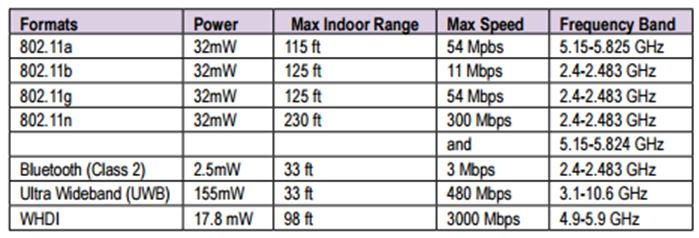
\includegraphics[width=\linewidth]{lit1.jpg}
	\caption{citeeeeeeeeeeeeeeeeeeeeee\cite{hall2015guyton}}
	\label{literaturereview1}
\end{figure}

\section{Wireless in Anaesthesia}

In the context of operating room, technical advances over the past decade have contributed to progress in anaesthesia safety. Improved patient monitoring, as well as increased usage of sensor system has introduced a new problem into practice, with great number of cables which makes care and nursing of patient difficult \cite{lit3}. 

Conventionally, sensors are wired to ensure uninterrupted monitoring of physiological variables. The use of wireless sensors will reduce the number of wires attached to the patients, easing transport and ambulation of patient in an intensive care environment \cite{lit2}. 

\section{Benefits}

There are many benefits associated with the use of wireless systems to measure vital signs in the operating theatre. First, the clutter of cables can be significantly reduced. The risk of contamination will also decrease as cables are often exposed to contamination and not easily cleaned before repeat exposure to a sterile field. In the long run, there will also be significant cost reductions associated to operating room renovations. Monitors are frequently damaged when operating room staff are required to connect and disconnect cables on a regular basis. The wear and tear of cables will also require replacement from time to time. Using wireless solutions will eliminate the need for cables completely. 

\begin{figure}[H]
	\centering
	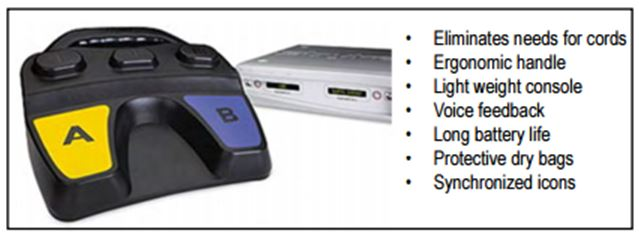
\includegraphics[width=0.7\linewidth]{lit2.jpg}
	\caption{Benefits of Wireless Monitoring Systems \cite{lit1}}
	\label{literaturereview2}
\end{figure}

For example, a wireless footswitch has been designed \cite{lit1} and this eliminates the need for cords to be draped around or placed on floor under the sterile field. It can also connect to the receiver simply and easily used by the operating room staff. This improves efficiencies, eliminate cables and obstacles reducing operating room hazards and improves the turnover rate of the operation room. 

\section{Challenges}

One of the main challenges associated with wireless monitoring systems would be security breach. It is a valid concern of someone snooping on data that is transmitted wirelessly. Adequate security and encryption have to be incorporated before it can be used in OR where a disruption of vital signs will be fatal. In the design of wireless antenna associated with the sensors, it is essential to ensure that consistent performance is achieved to avoid risk of affecting wireless range and quality of the wireless signal.  

Furthermore, interference may be a prevalent issue in wireless systems, especially when there are multiple different forms of communications existing at the same time. For example, the use of 2.4Ghz band can be crowded by WiFi and other RF traffic, which may result in noise in the signals. Using wireless technologies will also increase significant costs to the development and maintenance of the medical devices. 

\section{Priority Queueing Models}

As in our proposed model, there will be multiple sensors, namely EEG, ECG PPG etc. that are integrated into one transmission, a priority queueing model will need to be devised to ensure important vital signs data are prioritized when bandwidth / throughput is limited at certain stages of transmission. An appropriate queuing models are implemented to improve performance parameters for priority queueing, delay and server utilization time. In a study conducted by The NorthCap University \cite{lit4} indicate that using M/G/1 Or M/G/N queueing models will have better performance depending on the expected number of incoming packets. An extract of the results is shown below, serving as a reference to our queueing model. 

\begin{figure}[H]
	\centering
	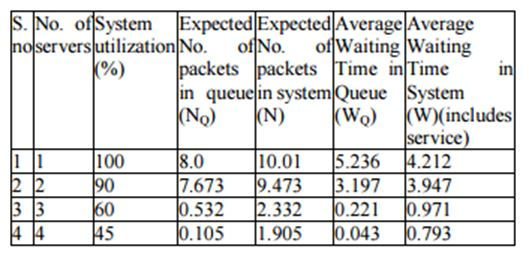
\includegraphics[width=0.7\linewidth]{lit3.jpg}
	\caption{Result for M/G/1 and M/G/N queueing models for the proposed scenario \cite{lit4}}
	\label{literaturereview3}
\end{figure}

\section{Case Studies}

There have been several successful studies that wirelessly monitors independent parameters but not all in the same package. For instance, in a project done in the University of Rhode Island \cite{lit3}, a smart wristband has been made to allow data transmission via bluetooth technology, which is able to send out BPM over standardized GATT Heart Rate Service that will calculate and output several metrics such as control point, heart rate etc. 

Wireless system that remotely monitors patient’s oxygen saturation (\%SPO2), pulse oximetry has also been devised \cite{lit5} In this project, researches have been able to transfer vital signs monitored by pulse oximeter via IEEE 902.15.4 to a wireless sensor network for storage and display. A preliminary evaluation of the proposed system indicates that it is medically satisfactory in terms of accuracy of data, validating the use of WLAN as a primary form of wireless networks. 

Case studies on Zigbee has also been done in India \cite{lit6}. By using Zigbee to monitor body temperature and heart rate, the team has managed to transmit vital parameters from body to all wirelessly connected computer. Zigbee was chosen due to convenience and cost effectiveness. However, the prototype has managed to send signals at 1Hz frequency and its power consumption is minimal. The downside is that the signal transmitted is susceptible to noise. Proof of concept of utilizing Zigbee has been established, but with limited throughput, it will not be sufficient for the arrays of data that will be transmitted in our project. 
 
With the emergence of 3D printed technology, it is possible to integrate it to design a scalable wireless monitoring system. A portable wireless systems measuring key metabolites in intensive care monitoring, using a 3d-printed case with sensing devices and integration of PCB with biosensors have been made in 2015, with successful implementation at its trials \cite{lit7}. The biosensors will then transmit its measurements via Bluetooth module to mobile Android interface. This indicate the possibility of using Android system as a universal display instead of individual displays for each of the separate sensors. 

Another solution that have been devised is to connect a dongle with wireless serial capability to convert serial data from some medical sensors to android devices such as smartphones for monitoring \cite{lit8}. This can be expanded to slave monitor, or even smart glasses in future novel applications. The use of smart devices as a platform to converge information of different sensors can also be used to recognize past trends to predict future trends, presenting a functionality of smart alarm. However, this approach do not solve the fundamental issue of Spaghetti Syndrome, but serves as a good design reference for setup of slave monitors in the Operating Room.

\section{Analysis of Existing Systems}

There are several biomedical wireless systems that have been devised for research purposes, and will be listed for comparison and benchmarking for our project. 

\subsection{Consideration of e-Health Sensor by Cooking Hacks (Libelium)}

The first would be the e-Health sensor shield, which is an interface with Arduino and Raspberry Pi to perform up to monitoring 10 different vital signs, including but not limited to SPO2, ECG, temperature, pulse etc \cite{lit9}.

\begin{figure}[H]
	\centering
	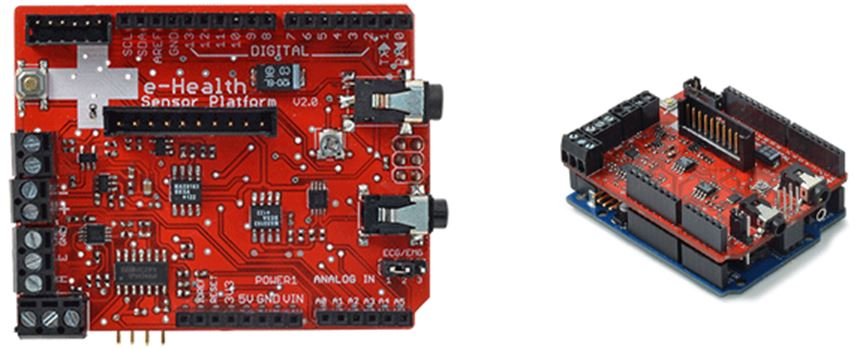
\includegraphics[width=0.7\linewidth]{lit4.jpg}
	\caption{e-Health Sensor Shield \cite{lit9}}
	\label{literaturereview4}
\end{figure}

This system is able to monitor the real time state of the patient to get sensitive data which can be subsequently used for analysis. Biometric information gather can be used to send wirelessly via multiple channel options: WiFi, 3G, GPRS, Bluetooth, 802.15.4 and Zigbee depending on application. However, this platform is designed to allow user to develop new products, i.e. an open source project to test different sensors and is not to be used in a professional medical context. 

A key takeaway from this product is the use of AES 128 for Zigbee transmission and use of WPA 2 protocol for Wifi transmission. This is important as medical data will require to be completely secure especially in the Operating Room, as a mishap in monitoring may result in fatalities.

\subsection{Consideration of BioNomadix Wireless Wearable Physiology by Biopac Systems}

Another existing system would be Bionomadix wireless wearable physiology from Biopac Systems. This is a system they are currently researching on and has developed their own platform where each BioNomadix modules can interface to \cite{lit10}. 

Each of the vital signs monitor(e.g. EEG, ECG) has separate transmitter and receiver, which makes the overall system to be bulky and harder to setup in a operating room. Contary to that, our design will allow integration of all sensors to one data transmission point, which reduces the total number of devices required for the same functionality. 

\begin{figure}[H]
	\centering
	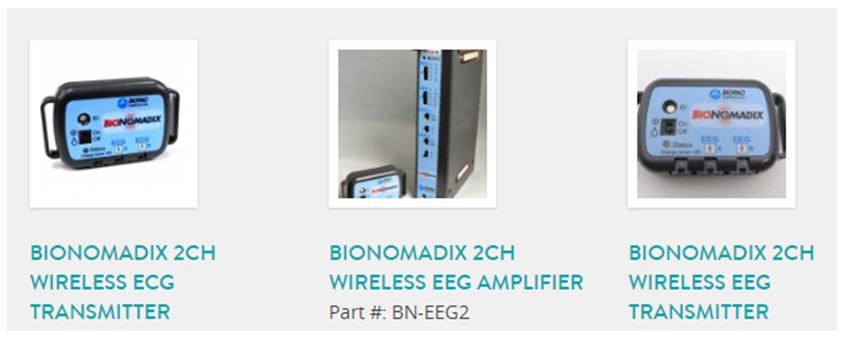
\includegraphics[width=\linewidth]{lit5.jpg}
	\caption{Sample of BioNomadix Separate Vital Sign Monitor \cite{lit10}}
	\label{literaturereview5}
\end{figure}






\section{Wireless Sensor Networks}

In line with the expansion of Internet of Things, this project is able to incorporate the idea of smart and ubiquitous connections between devices \cite{gubbi2013internet}.

\section{Body Area Networks}

\section{Methods of Wireless Transmission}

\subsection{Comparison between Virtual Nerwork Computing (VNC) and Raw Transmission}
\label{vnc}

One of the biggest considerations of the project is whether to transmit the raw data wirelessly or to allow access to the data-processing terminal via virtual network computing (VNC). A quick comparison between the strengths and weaknesses is laid out below, with reference to Figure \ref{system}. 

Raw data transmission from one terminal to another requires less processing power as the workload of data visualisation and transmission can be equally delegated between the two terminals. In terms of the actual transmission, the bandwidth required by raw data transmission is much smaller than the bandwidth needed for setting up and maintaining a VNC server-client connection. This directly implies that there would be a smaller delay for the raw data transmission model. 

On the other hand, VNC provides inherent encryption whereas raw data transmission is susceptible to interception if no encryption is implemented. In addition to this, most VNC server-client systems are packaged with user password authentication, providing increased security against unauthorised access to the sensor outputs collected from patients. Again, raw data transmission requires further deliberate work to attain similar security standards. 

In wireless systems, disconnection due to the devices going out of range is commonplace and can cause disruption in the flow of information between terminals. For a VNC implementation of the WVSMS, data-processing isolation is a great benefit obtained compared to raw data transmission. Referring to Figure \ref{system}, should a disconnection occur, data processing and visualisation are not interrupted as the wireless transmission component is a completely separate, independent, and disjointed process between the terminals. As such, the Terminal connected to the Sensors are completely isolated. The Display-connected Terminal is not required for the system to function as the purpose of the second Terminal is only to be a VNC client for accessing the first Terminal. However, for raw data transmission be interrupted, both data processing and visualisation (assuming this is done by the Display-connected Terminal), will terminate completely due to the cessation of input. Using a VNC model effectively eliminates the problem of transmission errors affecting data processing.  

Another point worth noting is the full remote control of the Sensor-connected Terminal that VNC affords to the user should there be a need to access the Terminal in real time to operate and change the processes. Raw transmission does not allow such control between Terminals. 

From the above comparison, it can be seen that using VNC is highly suited for the purposes of this project instead of raw data transmission according to the required specifications as seen in Section \ref{specifications}. \\

\subsection{Virtual Network Computing}


https://en.wikipedia.org/wiki/Virtual\_Network\_Computing 

VNC is platform-independent 

VNC
encryption
isolation - big point
security - authentication
full remote control over patient's devices 

Raw 
Less processing power required
Less delay

\section{WiFi}

\section{Bluetooth}

\section{Zigbee}

\section{Comparison of Different Protocols}

\begin{center}
	\begin{tabular}{| l | l |}
		\hline
		Test1 & Test2 \\ \hline
	\end{tabular}
\end{center}
	
	\chapter{Project Design and Development}


\section{System Overview}

The hardware of this vital signs monitoring system has been divided into three major sections as seen in Figure 3.1, namely: 

\begin{itemize}
	\item Sensors - Collects raw measurements of separate vital sign parameters 
	\item Terminals - Processes data and handle transmission/reception of information
	\item Display - Visualises output of critical vital sign information
\end{itemize}

A block diagram of the Wireless Vital Signs Monitoring System is shown in Figure \ref{system} down below. The system consists of three major portions: the Sensors which collect the raw measurements of separate vital sign parameters, the Terminals which process the data and handle transmission/reception of information, and the Display which visualises the output. The details of the development and options considered for each portion are further described in Sections \ref{terminals}, \ref{sensors}, and \ref{processing}.

\begin{figure}[H]
	\centering
	\includegraphics[width=\linewidth]{system2.png}
	\caption{Wireless Vital Signs Monitoring System Block Diagram}
	\label{system}
\end{figure}

\section{Design Specifications}
\label{specifications}

\section{Hardware Design and Development}







\section{Software Design and Development}
\label{software}




\section{Analysis of Competitors - Similar Papers - Literature Review}







\section{Analysis of Existing Systems}

\subsection{Consideration of Bionomadix}

\subsection{Consideration of Libelium and Waspmote}

\subsection{Consideration of Cooking Hacks}

	\chapter{Terminals for Data Processing} 
\label{terminals}

The {\bf Terminal} or {\bf Platform} in this report refers to the machine or computer (hardware) which handles the processing of the raw measurements acquired from the sensors, the visualisation of the data received, in addition to the transmission and reception of the information from one geographical location to another through electromagnetic waves. Multiple types of terminals were considered and the factors which were accounted for were:

\begin{enumerate}
	\item Processing Power
	\item Operating System
	\item Price
	\item Power Consumption
	\item Wireless Capabilities
	\item Number of Input/Output Ports
\end{enumerate} 

\section{Operating System}
\label{os}

Of all the factors mentioned above, the OS for the Terminal is the most important and deserves a section of its own for further discussion. The OS must be fully capable of running the software required for data processing, data visualisation, virtual network computing (VNC) server hosting, and wireless transmission. Consequently, the OS determines which Terminal should be chosen as some platforms are designed based on a specific OS.  

Based on the above criteria, Linux was chosen for this project due to the open source nature of the OS. Many software programs and applications required for the functionality specified, such as the ones mentioned in Section \ref{software}, are readily available without cost from the Linux software database. Despite being an open source technology, security is not a concern but on the contrary, a significant advantage \cite{linuxadvantagedisadvantage}. By releasing the source code of the OS to the general public, security experts from various backgrounds and fields are able to identify major security flaws in the system \cite{linuxadvantagedisadvantage}. This allows for the swift resolution of such breaches by developers around the world, making security issues nullified as soon as they are found. Unlike proprietary OS such as Windows, the international community of developers are the ones who maintain the system for Linux, rather than a fixed number of employees working in specific locations around the world.  

Nevertheless, one substantial problem with Linux OS is drivers for new hardware components \cite{linuxadvantagedisadvantage}. However, due to the lower level nature of this project, drivers can be developed and so does not pose a major threat. Other drivers required for microcontrollers such as the Arduino Uno/Arduino Pro Mini for analogue to digital conversion are readily available and hence, does not pose a major threat.  

One such platform which runs on a Linux kernel is the Rasberry Pi 3. The Linux distribution which was suggested by default for this miniaturised computer is the Raspbian Jessie, which is the Raspberry Pi derivative of the long standing Debian distribution. Section \ref{rpi} has been dedicated to further analyse the Raspberry Pi 3 Model B used for this project. 

Having a platform that runs on a Linux kernel provides the significant advantage of the ease of migration. As the project is a pilot study in wireless vital signs monitoring systems, there is a foreseeable need to continuously upgrade the platforms in terms of hardware capabilities to accommodate other important features. As long as the Linux kernel is used, it is not difficult to migrate to another more powerful Linux-based platform as the applications database and drivers available do not greatly differ for specific Linux distributions. \\


of all these, the OS is the most important - deserves a section of its own for discussion
very important - terminal is chosen based on this

Raspbian Jessie - Linux kernel - open source - more software and support available 

- ease of migrating to other platforms - as long as the kernel remains the same 

- windows considered -but proprietary - software will be expensive - issues if no support - limited support - need for payment

linux provides 
\cite{linuxwindows}

\section{Raspberry Pi 3 Model B}
\label{rpi}

Based on the criteria set out in Section \ref{os}, the Raspberry Pi 3 Model B loaded with a Raspbian Jessie OS is chosen as the platform or terminal for the project, henceforth referred to as the \textbf{Raspberry Pi}.

\begin{figure}[H]
	\centering
	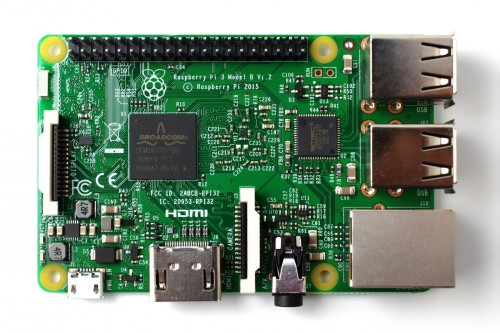
\includegraphics[width=0.7\linewidth]{rpi3.jpg}
	\caption{Raspberry Pi 3 Model B \cite{rpi3pic}}
	\label{rpi3pic}
\end{figure}


\cite{rpi3mb}

The specifications of the Raspberry Pi 3 Model B are as follows \cite{rpi3mb}: 
\begin{itemize}
	\item 1.2GHz 64-bit quad-core ARMv8 CPU
	\item 802.11n Wireless LAN
	\item Bluetooth 4.1
	\item Bluetooth Low Energy (BLE)
	\item 1GB RAM
	\item 4 USB ports
	\item 40 GPIO pins
	\item Full HDMI port
	\item Ethernet port
	\item Combined 3.5mm audio jack and composite video
	\item Camera interface (CSI)
	\item Display interface (DSI)
	\item Micro SD card slot (now push-pull rather than push-push)
	\item VideoCore IV 3D graphics core
\end{itemize}

The Raspberry Pi's CPU is capable of running different types of Linux-based OS, in particular, ARM Linux distributions. Examples of such OS are Raspbian and Ubuntu Mate, whereas an instance of a non-Linux-based OS is the Windows 10 IoT Core. As discussed in Section \ref{os}, it is preferable to use the Raspbian Jessie as it is designed specifically for the Raspberry Pi. 

In terms of connectivity, the Raspberry Pi leaves little to be desired with an integrated 802.11n Wireless LAN. This inbuilt WiFi adapter provides the needed wireless interface for the WVSMS and lays the foundation of the project back end design. An Ethernet port is also available as a contingency for reliable operation. 

The 4 USB ports and 40 GPIO pins allow the sensors to be connected to the Terminal. However, it is important to note that all GPIO pins on the Raspberry Pi are only for digital input and output. Due to the absence of the analog-to-digital converters, there is a need to implement an interface for the Sensors, which provide signals in analog form. This is done using the Arduino Uno/Arduino Pro Mini as seen in Section \ref{arduino}. 

The full HDMI port and VideoCore IV 3D graphics core provides the graphic processing power required to render the images when data is visualised and displays it to a monitor. 

Based on the criteria laid out in Section \ref{terminals}, the Raspberry Pi provides the necessary processing power, operating system, power consumption, wireless capabilities, and input/output ports at a reasonable price. 

The schematic design of the Raspberry Pi 3 Model B can be found in Appendix \ref{rpi3bschematic}.

\cite{rpi3hardware}


\subsection{Raspbian Jessie}

Raspbian Jessie is 
\cite{rpi3raspbian}
https://www.raspbian.org/

Installation instructions can be found in Appendix \ref{appraspbianjessie}


Version:May 2016
Release date:2016-05-27
Kernel version:4.4


\subsection{Portable Power Supply for the Raspberry Pi 3 Model B}
\cite{rpi3faqs}

The Raspberry Pi is powered using a 5V micro-USB power supply\cite{rpi3faqs}. The current drawn by the Raspberry Pi is variable and depends on the applications running in addition to the current drawn by peripheral devices which are connected. Typically, the Raspberry Pi 3 Model B current requirements range from 1.2A to 2.5A \cite{rpi3faqs}. 

Buck - 9V

\section{Intel Nuc}


	\chapter{Sensors} 
\label{sensors}

The {\bf Sensors} in this report refer to the separate sensors connected to the body of the patient which collects raw measurements of vital sign paramaters, conditions the data so that it is suitable for analogue to digital conversion, and converts the data into a digital signal that can be interpreted by the platform ({\bf Terminals}). \\

The sensors used in this project are enumerated as follows with the respective vital sign parameter measured: 

\begin{enumerate}
	\item ECG - AD8232 Heart Rate Monitor 
	\item PPG - 
	\item EEG - 
	\item Blood Pressure - 
	\item Blood Temperature - Thermistor coupled with Phase Shift Oscillator
\end{enumerate}

The following sections below further discusses the reason behind the choices made for the individual sensors, the mechanism of operation, and how it interfaces with the entire system. 

\section{ECG}

The ECG front end design consists of a number of parts. 

The typical range of an ECG signal lies between $0.01\sim 300Hz$ and $0.05\sim 3mV$ in terms of frequency and amplitude respectively \cite{nisignalamplitude}. The voltages sampled from the surface of the skin through electrodes are too miniscule to be directly plotted and displayed. In addition, there are multiple frequencies which are of interest in ECG signals but the raw measurements will contain unwanted signal artifacts from other sources. Hence, it is necessary to amplify and filter the signal before any analysis or visualisation is performed.  

In 1997, Strohmenger \cite{strohmenger1997analysis} did an analysis of ventricular fibrillation ECG signal amplitude and frequency parameters for both successful and unsuccesful cardiac arrest countershocks. In this paper, the frequency range and amplitude range of both cases corroborates with the typical values stated above.  



\subsection{AD8232 IC ECG Sensor}

In this project, in line with the aim of producing a system that is a working proof of concept, a simplified version of the ECG is used. The AD8232 IC from Analog Digital was used \cite{ad8232datasheet}. 

\subsubsection{Front End}

The Analog Devices AD8232 was used to implement the ECG part of this project. The AD8232 is "an integrated signal conditioning block for ECG", "designed to extract, amplify, and filter small biopotential signals" \cite{ad8232datasheet}. The functional block diagram is included below in Figure \ref{ad8232functional}. 

\begin{figure}[H]
	\centering
	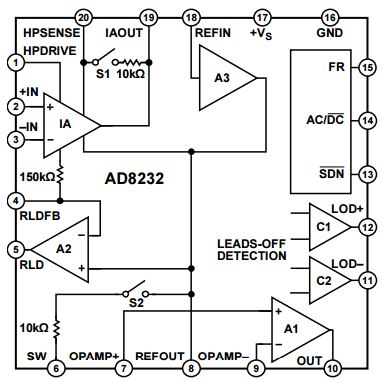
\includegraphics[width=0.5\linewidth]{ad8232funcdiagram.jpg}
	\caption{AD8232 Functional Block Diagram \cite{ad8232datasheet}}
	\label{ad8232functional}
\end{figure}

\begin{figure}[H]
	\centering
	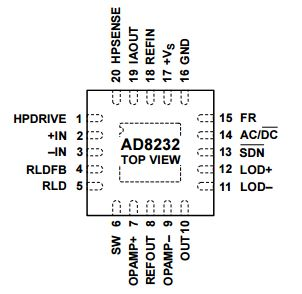
\includegraphics[width=0.4\linewidth]{ad8232pin.jpg}
	\caption{AD8232 Pin Configuration \cite{ad8232datasheet}}
	\label{ad8232pin}
\end{figure}

\subsubsection*{Theory of Operation of the AD8232}

\begin{figure}[H]
	\centering
	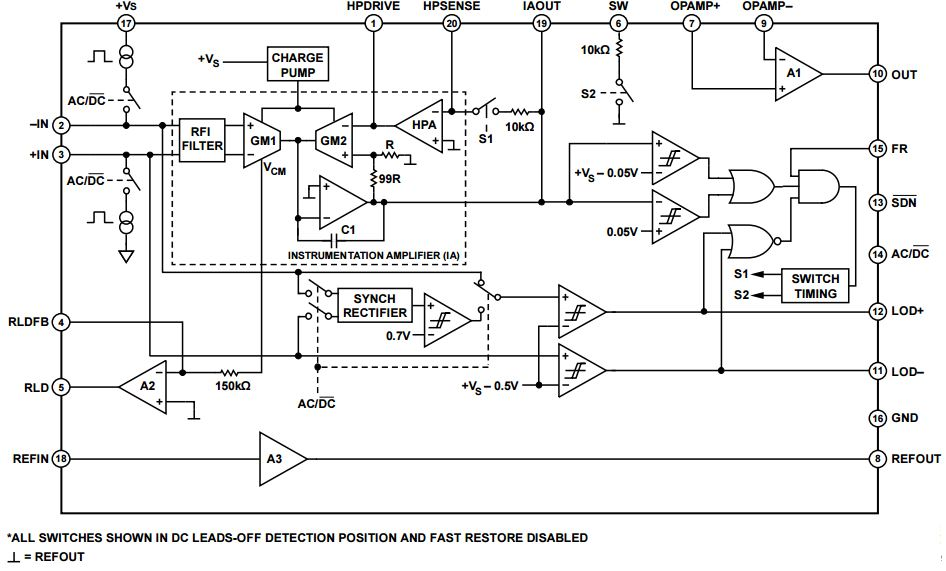
\includegraphics[width=\linewidth]{ad8232schematic.jpg}
	\caption{AD8232 Simplified Schematic Diagram \cite{ad8232datasheet}}
	\label{ad8232schematic}
\end{figure}

Figure \ref{ad8232schematic} above shows the architectural overview of the AD8232 chip from Analog Devices used for the "front end signal conditioning of cardiac biopotentials" \cite{ad8232datasheet} and is comprised of the following components: 

\begin{itemize}
	\item Specialized instrumentation amplifier (IA) - Amplifies ECG signals 
	\item Operational amplifier (A1) - For low pass filtering and supplying extra gain 
	\item Right leg drive amplifier (A2) - Improves common-mode signal rejection by inverting the signal 
	\item Midsupply reference buffer (A3) - Provides a reference signal for the IA by creating a virtual ground between the supply voltage and system ground 
	\item Leads off detection circuitry - Senses and indicates if the electrodes have been disconnected
	\item Automatic fast restore circuit - Decrease settling time of the ECG signal for a quicker response 
\end{itemize} 

\cite{ad8232analogdevices}

\cite{ad8232evalzuserguide}

\cite{ad8232datasheet}

\subsubsection*{AD8232 IC Cardiac Monitor Circuit Configuration}

The datasheet for the AD8232 provided by Analog Devices supplies a typical circuit setup and configuration for a cardiac monitoring as seen in the schematic diagram in Figure \ref{ad8232cardiacconfig} below \cite{ad8232datasheet}. A printed circuit board with this configuration could have been assembled and constructed using Altium Designer but due to time and cost constraints, an exact implementation of this circuit (with additional headers, an LED indicator, and a 3.5mm jack for biomedical pad connection) from SparkFun Electronics was used instead \cite{ad8232}.   

\begin{figure}[H]
	\centering
	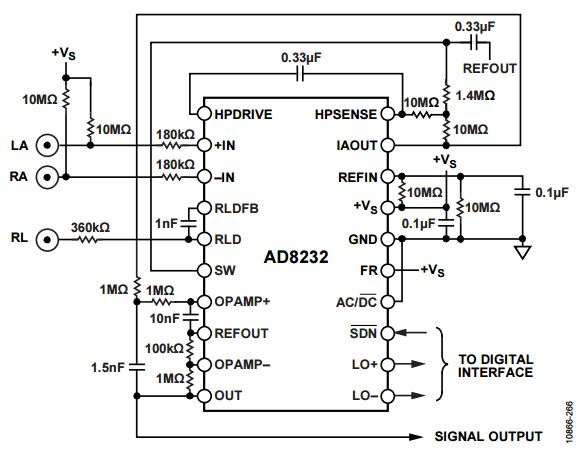
\includegraphics[width=0.7\linewidth]{ad8232cardiacconfig.jpg}
	\caption{Circuit Configuration for ECG Waveform Monitoring using the AD8232 \cite{ad8232datasheet}}
	\label{ad8232cardiacconfig}
\end{figure}
 
The schematic of the actual schematic capture of the AD8232 by SparkFun can be found in Appendix \ref{ad8232sfschematic}. The AD8232 Heart Monitor in Figure \ref{ad8232sfboard} is essentially a breakout board for the AD8232 integrated circuit provided by Analog Devices. 

\begin{figure}[H]
	\centering
	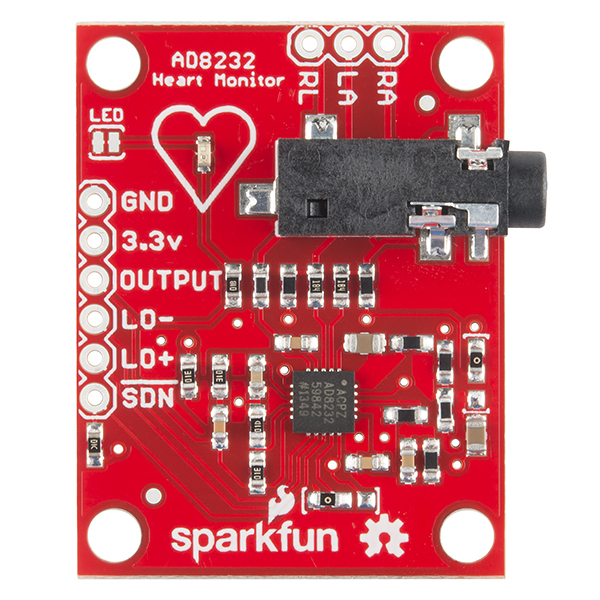
\includegraphics[width=0.4\linewidth]{ad8232sfboard.jpg}
	\caption{AD8232 Heart Rate Monitor from SparkFun Electronics \cite{ad8232}}
	\label{ad8232sfboard}
\end{figure}

CONSIDER PUTTING ALTIUM DESIGNER DESIGN

\subsubsection*{Complete AD8232 ECG Sensor Setup}

Due to the absence of an analog-to-digital converter, it is necessary to use a microcontroller which is capable of this conversion and serial communication through a USB port for prototyping. As such, an Arduino Pro Mini 328 (3.3V/8MHz) was used in the development of the interface. The design of the system was sourced from SparkFun Electronics \cite{ad8232}. 

The assembly of the complete AD8232 ECG sensor requires the following components \cite{ad8232}:

\begin{enumerate}
	\item Arduino Pro Mini 328 - 3.3V/8MHz (DEV-11114)
	\item SparkFun USB Mini-B Cable - 6 foot (CAB-11301)
	\item SparkFun FTDI Basic Breakout - 3.3V (DEV-09873)
	\item Break Away Headers - Straight (PRT-00116)
	\item Sensor Cable - Electrode Pads (3 connector) (CAB-12970)
	\item Biomedical Sensor Pad (10 pack) (SEN-12969) 
	\item SparkFun Single Lead Heart Rate Monitor - AD8232 (SEN-12650) 
\end{enumerate}

These components are assembled in the pattern found in Figure \ref{ad8232sffritzing}. 

\begin{figure}[H]
	\centering
	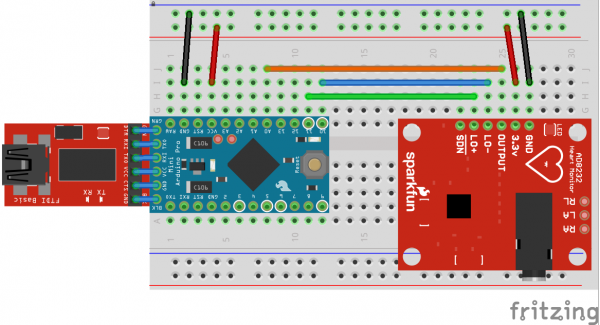
\includegraphics[width=0.9\linewidth]{ad8232fritzing.png}
	\caption{AD8232 Connection Diagram using Fritzing \cite{ad8232}}
	\label{ad8232sffritzing}
\end{figure}

In terms of the pin connections between the AD8232 and the Arduino Pro Mini, the connections are found in Table \ref{ad8232pinconfigurationtable}.

\begin{table}[H]
	\centering
	\caption{Pin Configuration for the AD8232 and the Arduino Pro Mini \cite{ad8232}}
	\label{ad8232pinconfigurationtable}
	\begin{tabular}{|l|l|l|}
		\hline
		\textbf{Board Label} & \textbf{Pin Function} & \textbf{Arduino Connection} \\ \hline
		GND                  & Ground                & GND                         \\ \hline
		3.3v                 & 3.3v Power Supply     & 3.3v                        \\ \hline
		OUTPUT               & Output Signal         & A0                          \\ \hline
		LO-                  & Leads-off Detect -    & 11                          \\ \hline
		LO+                  & Leads-off Detect +    & 10                          \\ \hline
		SDN                  & Shutdown              & Not used                    \\ \hline
	\end{tabular}
\end{table}


The complete circuit can be found in the Figure below 

FIGUREEEEEEEEEEEEEEEEEEEEEEEEEEEEEEEEEEEEEEEE

To circumvent the need of using a breadboard, a PCB shield for the AD8232 and the Arduino Pro Mini was designed to accomodate both breakout boards on a single board without the need for wires to connect the internal components. The PCB design can be found in Appendix \ref{ecgshieldpcb}. 

- Uploaded and compiled sample Arduino code from SparkFun GitHub repository. 
- Need to change board type to Arduino Pro Mini 328 - 3.3V/8MHz. 



\section{Blood Temperature}

\subsection{Thermistor}

One of the methods to measure body temperature is through measuring heat conduction via direct physical contact with the patient's body. As a thermistor is a temperature-dependent resistor, the resistance of a thermistor varies with temperature. The property of thermistors therefore, are desirable in the design of a temperature sensor. 

Using an Arduino Uno for prototyping, a simple voltage divider is constructed to study the characteristics of a thermistor. The thermistor used in this project is a material type F thermistor \cite{thermistor}. The circuit in Figure \ref{temperaturefritzing1} was constructed for testing the thermistor. 

\begin{figure}[H]
	\centering
	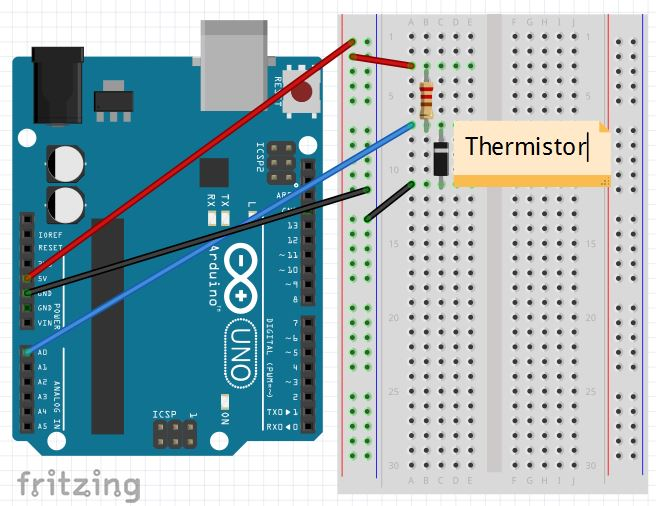
\includegraphics[width=0.5\linewidth]{temperaturefritzing1.jpg}
	\caption{Thermistor in Voltage Divider Configuration using Fritzing}
	\label{temperaturefritzing1}
\end{figure}

The datasheet of the material type F thermistor \cite{thermistor} reveals the following formulae and properties: 

\begin{figure}[H]
	\centering
	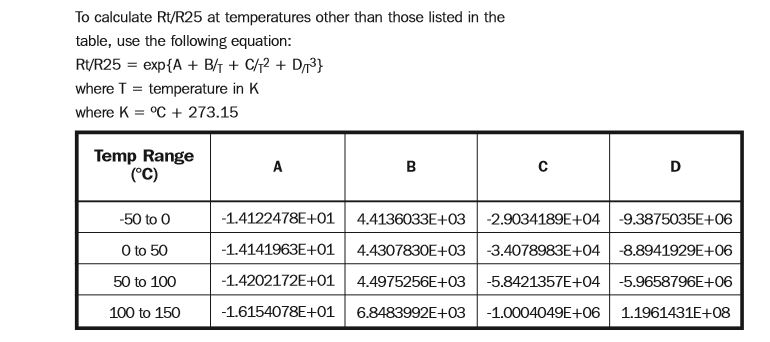
\includegraphics[width=0.8\linewidth]{thermistordatasheet2.jpg}
	\caption{Thermistor Formulae and Properties \cite{thermistor}}
	\label{thermistordatasheet2}
\end{figure}

\begin{figure}[H]
	\centering
	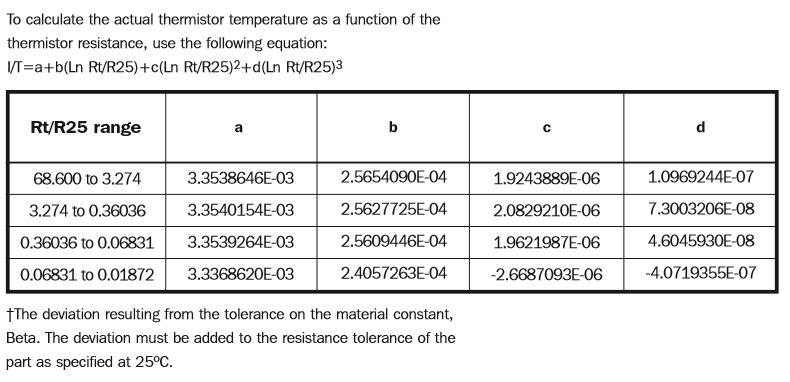
\includegraphics[width=0.8\linewidth]{thermistordatasheet3.jpg}
	\caption{Thermistor Formulae and Properties (cont.) \cite{thermistor}}
	\label{thermistordatasheet3}
\end{figure}

\begin{equation}
	\frac{Rt}{R25} = exp(A+\frac{B}{T}+\frac{C}{T^2}+\frac{D}{T^3}) 
	\label{thermistorresistance1}
\end{equation}

\begin{equation}
	\frac{1}{T} = a+b(ln\frac{Rt}{R25})+c(ln\frac{Rt}{R25})^2+d(ln\frac{Rt}{R25})^3\\
	\label{thermistorresistance2}
\end{equation}

T is the temperature in Kelvin where $K=\degree C+273.15$. 

Choosing an operating temperature range of $0\degree C$ to $50\degree C$, Equation \ref{thermistorresistance1} and \ref{thermistorresistance2} has the following parameters: 

\begin{table}[H]
	\centering
	\caption{Material Type F Thermistor Parameters for $0\degree C$ to $50\degree C$}
	\label{thermistorparameters}
	\begin{tabular}{|l|l|}
		\hline
		A = -1.4141963E+01  & a = 3.3540154E-03 \\ \hline
		B = 4.4307830E+03   & b = 2.5627725E-04 \\ \hline
		C = -3.40789983E+04 & c = 2.0829210E-06 \\ \hline
		D = -8.8941929E+06  & d = 7.3003206E-08 \\ \hline
	\end{tabular}
\end{table}

Therefore, we know that the range of $\frac{Rt}{R25}$ is between 0.36036 to 3.274. $R_{25}$ was chosen to be $10k\Omega$. This circuit was tested with the Arduino code found in Appendix \ref{arduinothermistor}.





It is also known that this material type F thermistor is a negative temperature coefficient (NTC) thermistor, that is, when the temperature rises, there is a decrease in resistance. 

\subsection{Self-Heating - Phase Shift Oscillator}

How does the phase shift oscillator actually work

How does the PSO help in reducing self-heating
Frequency becomes temperature dependent - Voltage not high across the thermistor 

PSO - Bipolar transistor Implementation \cite{psotutorial}

\subsection{Astable Operation of 555 Timer}

Another method of signal condition for the thermistor involves using the 555 Timer in astable operation. 

555 Timer Datasheet. 

\section{Interface}

\subsection{USB}

\subsection{Arduino Uno / Arduino Pro Mini - Analog to Digital Conversion}
\label{arduino}

Arduino Pro Mini 328 - 3.3V/8MHz

\subsubsection{Sensitivity of Arduino Uno} 

1023 bits
	\chapter{Data Processing, Visualisation, and Transmission} 
\label{processing}

The following programs are required for the complete functionality of the WVSMS using the Raspberry Pi Terminals running on Raspbian Jessie: 

\begin{itemize}
	\item \textbf{Tight VNC Server} - Set up VNC server required to access the Raspberry Pi with its internal programs and applications \cite{rpitightvncserver}.
	\item \textbf{X Tight VNC Viewer} - Allows the Display-connected Terminal to access and view the Sensor-connected Terminal via the VNC server	\cite{rpitightvncserver}.
	\item \textbf{Arduino} - Provides analog-to-digital interface between Sensor and Terminal, converts the signal into a serial input for processing, and visualisation \cite{arduino}.
	\item \textbf{Matplotlib} - Software which renders graphs from text files \cite{matplotlib}.
	\item \textbf{Processing 2.2.1} - Software sketchbook which receives serial inputs and renders real-time graphs of given information \cite{processing221}.
	\item \textbf{Java 7} - Allows Java-based applications to run on the Platform (specifically required for Processing 2.2.1) \cite{java7}.
\end{itemize}


\begin{lstlisting}
sudo apt-get update
sudo apt-get install tightvncserver
sudo apt-get install xtightvncviewer
sudo apt-get install arduino
sudo apt-get install python-matplotlib
\end{lstlisting}

\begin{lstlisting}
curl https://processing.org/download/install-arm.sh | sudo sh
\end{lstlisting}




- Also, need to use Processing 2.2.1, not 3.1.1. 
- Devices will not function with new version of Processing, displaying size() error. 
- Might be necessary to uninstall package 'libgles2-mesa' before using Processing, to prevent startup errors related to the P2D and P3D renderers. 
- Downloaded Processing 2.2.1 from https://processing.org/download/?processing for Linux 32 platforms. 
- processing-2.2.1-linux32.tgz is a 98.4 MB file. 


\begin{lstlisting}
sudo apt-get update'
sudo apt-get install oracle-java7-jdk
sudo update-alternatives --config java
\end{lstlisting}




- Processing 2.2.1 runs well on Java 7, not Java 8. 
- By default the Raspbian Jessie ships with Java 8. 
- Need to install Java 7 using the following commands: 
1. 'sudo apt-get update'
2. 'sudo apt-get install oracle-java7-jdk' 
3. 'sudo update-alternatives --config java'
- Extracted the tar file using 'tar xvzf processing-2.2.1-linux32.tgz'. 
- Need to remove the x86 Java runtime and replace with RPi armhf version. Use: 
1. 'rm -rf ~/processing-2.2.1/java
2. 'ln -s /usr/lib/jvm/jdk-7-oracle-armhf ~/processing-2.2.1/java'




- 'ln -s /usr/lib/jvm/jdk-7-oracle-armhf ~/processing-2.2.1/java' does not work. Folder name is different. 
- Copy '/usr/lib/jvm/jdk-7-oracle-arm-vfp-hflt' to the 'java' folder in processing-2.2.1. 
- Change 'myPort = new Serial(this, Serial.list()[1], 9600);' depending on which serial port is used. 


\section{Processing 2.2.1}

\section{Serial Input}

\section{Code}




\section{Visualisation}

\section{Wireless Transmission}
 
For this project, wireless communications between the Sensor-connected Terminal and the client requires the use of VNC as seen in Section \ref{vnc}. 

To set up the Raspberry Pi as a VNC server, TightVNCServer was used . For the Windows client used to access the VNC server of the Raspberry Pi, Tight VNC Viewer was used \cite{windowstightvnc}. 


	
\chapter{Simulation}
\label{simulation}

In the early phases of development, it was necessary to simulate the ECG signals as inputs into the system to observe both how the signals would be transmitted (through raw data transmission), and the typical form of the output waveform. To achieve this, an ECG signal was produced and plotted in MATLAB using the code from PhysioNet which can be found in Appendix \ref{ecgsimulationcode} \cite{ecgsimulation}.

\begin{figure}[H]
	\centering
	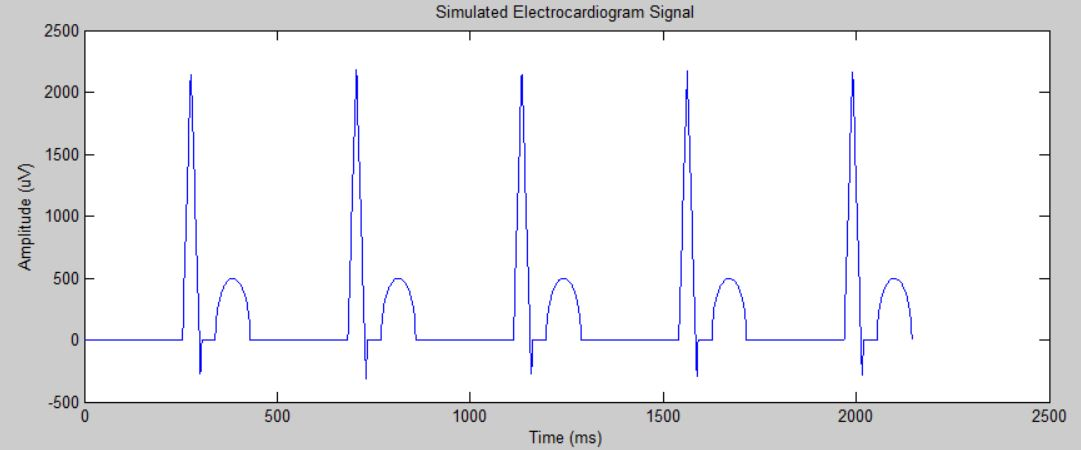
\includegraphics[width=\linewidth]{ecgsim.jpg}
	\caption{Simulated ECG Signal}
	\label{ecgsim}
\end{figure} 

\chapter{Testing}
wireless VNC

\chapter{Results}

\section{Wireless Vital Signs Monitoring System}

\subsection{Setup}

\section{Interface Output}



\section{ECG}

\subsection{AD8232 and Arduino Pro Mini Setup}



\subsection{ECG Electrode Placement}
For normal ECG systems, 10 cables are sufficient to acquire and display 12 electrical perspectives of the heart \cite{ashley2004conquering}. The typical attachment sites are found in Figure \ref{standardattachment} below. 

\begin{figure}[H]
	\centering
	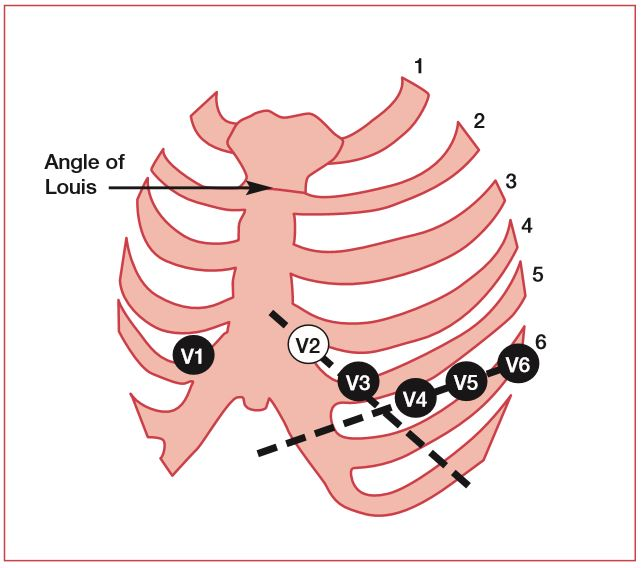
\includegraphics[width=0.5\linewidth]{standardattachment.jpg}
	\caption{Typical Sensor Placements 
		\cite{ashley2004conquering}}
	\label{standardattachment}
\end{figure} 

The AD8232 Heart Rate Monitor from SparkFun Electronics \cite{ad8232} provides three separate sensor pads and should be located in close proximity to the right arm, left arm, and the right leg, as seen in Figure \ref{sensorplacement} below. 

\begin{figure}[H]
	\centering
	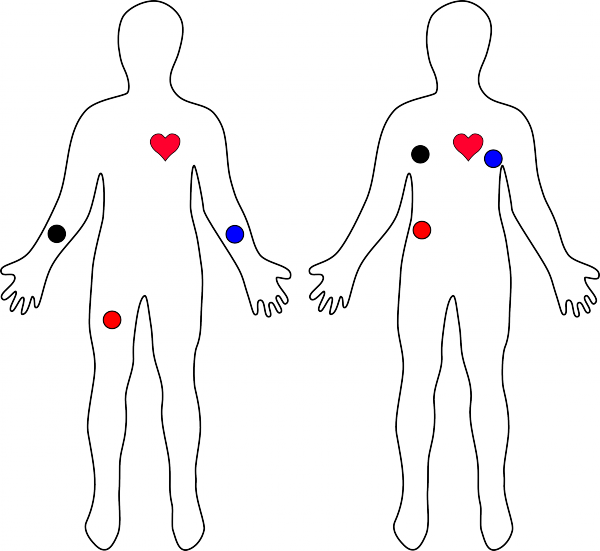
\includegraphics[width=0.5\linewidth]{body.png}
	\caption{Typical Sensor Placements (3 Electrodes)
	\cite{ad8232}}
	\label{sensorplacement}
\end{figure} 

In compliance with the suggested sites of sensor attachments, the approximate position of the electrodes are: 

\begin{itemize}
	\item 1 inch above the right nipple
	\item 1 inch above the left nipple
	\item 2.5 inches right of the navel
\end{itemize}

\subsection{ECG Output}

When initially operating the AD8232 Heart Rate Monitor, the ECG waveform output was not in the form of a recognisable heartbeat as seen in Figure \ref{ecgtest2}. Several adjustments were necessary to reduce noise in the ECG output and to capture the heartbeat waveform. 

\begin{figure}[H]
	\centering
	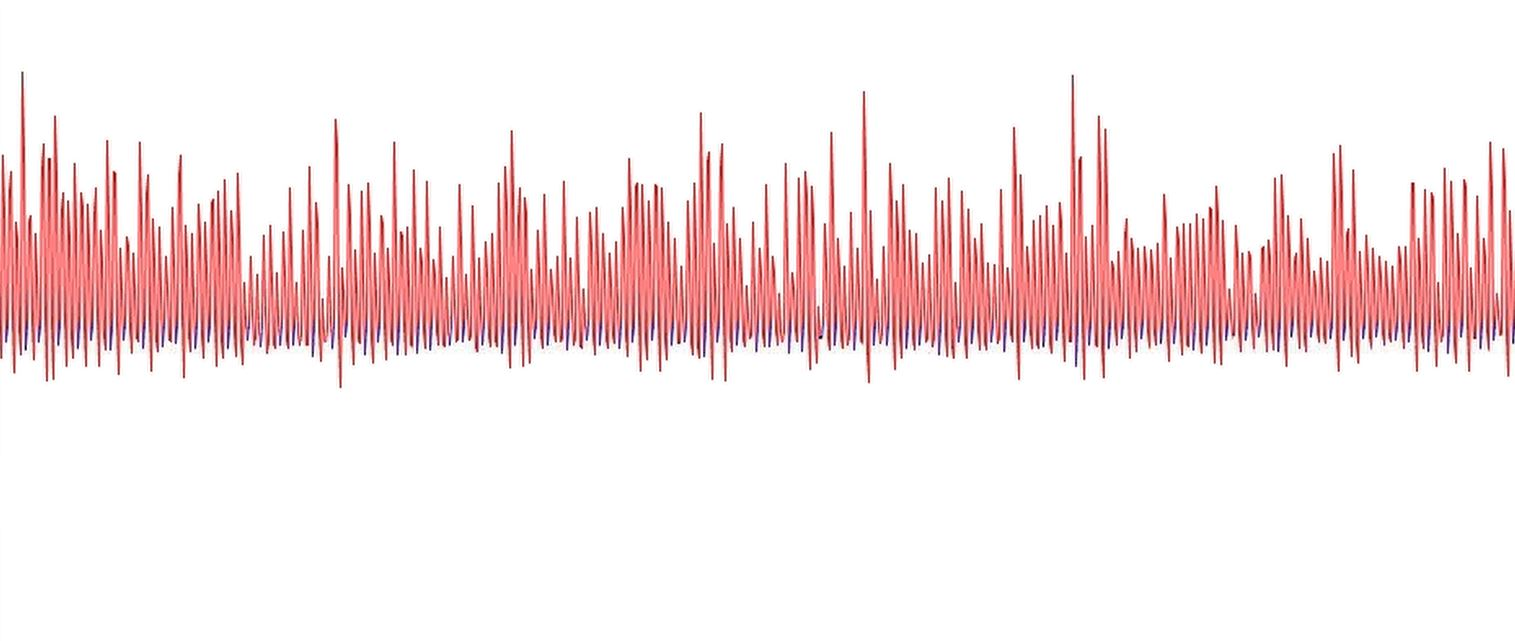
\includegraphics[width=\linewidth,height=40mm,frame]{ecgtest2.jpg}
	\caption{ECG Output Test 2}
	\label{ecgtest2}
\end{figure} 

When conducting the experiments, it is noted that the ECG output is significantly affected by posture and position of the body. This is explained more in Section \ref{motionartifact}. The best results were obtained from an upright sitting position with hands resting in front on a horizontal platform. 

\begin{figure}[H]
	\centering
	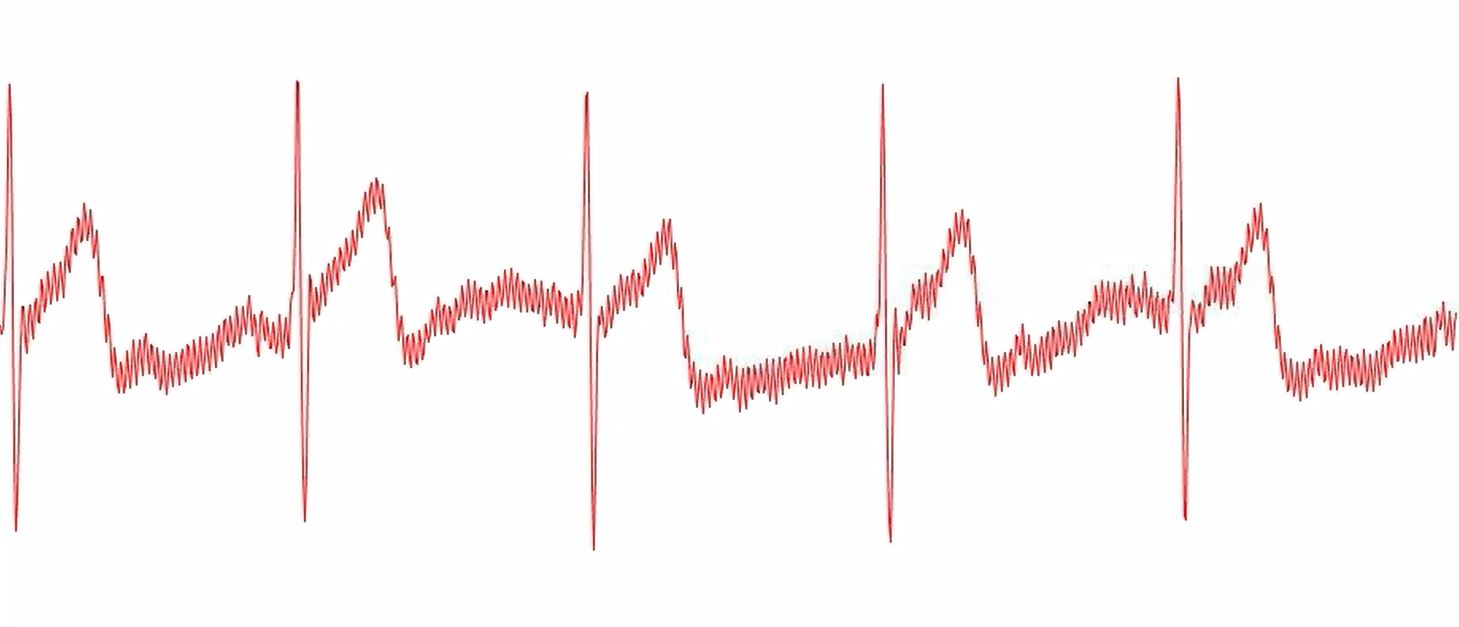
\includegraphics[width=\linewidth,height=40mm,frame]{ecgtest19.jpg}
	\caption{ECG Output recorded by the Raspberry Pi over WiFi}
	\label{ecgoutput}
\end{figure} 

\subsection{Motion Artifacts} \label{motionartifact}
At its core, ECG records electrical activity from muscle contractions through electrodes located on the skin \cite{ashley2004conquering}. As such, ECG systems are significantly affected by muscle contractions regardless of its origin. In measuring heart electrical activity, it is inevitable that electrical signals from other muscles in the body will be registered by the ECG system. Therefore, the output of ECG systems are highly variable and extremely susceptible to muscle movement, which introduces unwanted noise into the heart ECG output. This includes deep breathing or any movement of limbs while measurements are taken. 

The AD8232 cardiac circuit configuration from the datasheet "assumes that the patient remains relatively still during the measurement, and therefore, motion artifacts are less of an issue" \cite{ad8232datasheet}.

Figure \ref{ecgbreathing} illustrates how breathing can affect the vertical axis of the ECG output. 

\begin{figure}[H]
	\centering
	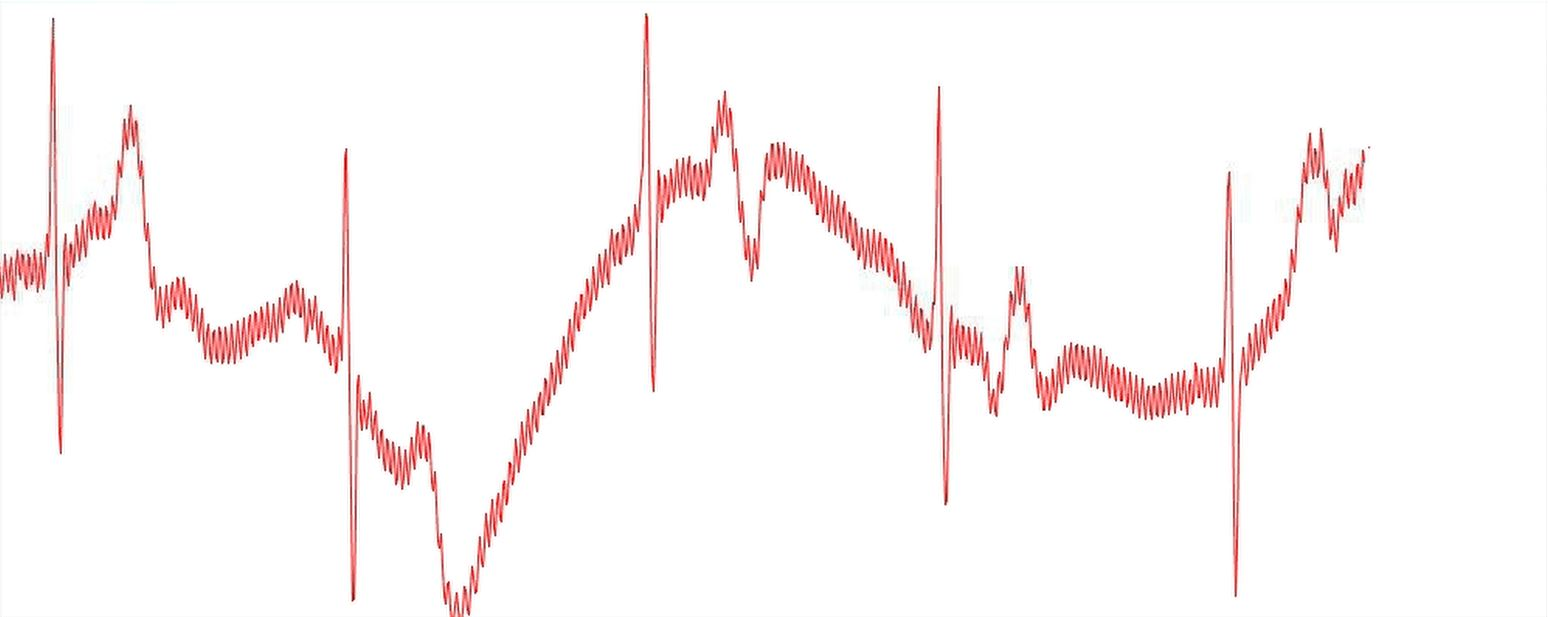
\includegraphics[width=\linewidth,height=40mm,frame]{ecgtest12.jpg}
	\caption{ECG Output with Deep Breathing}
	\label{ecgbreathing}
\end{figure} 

Figure \ref{ecgmovement} illustrates how moving limbs can affect the output of the ECG system. 

\begin{figure}[H]
	\centering
	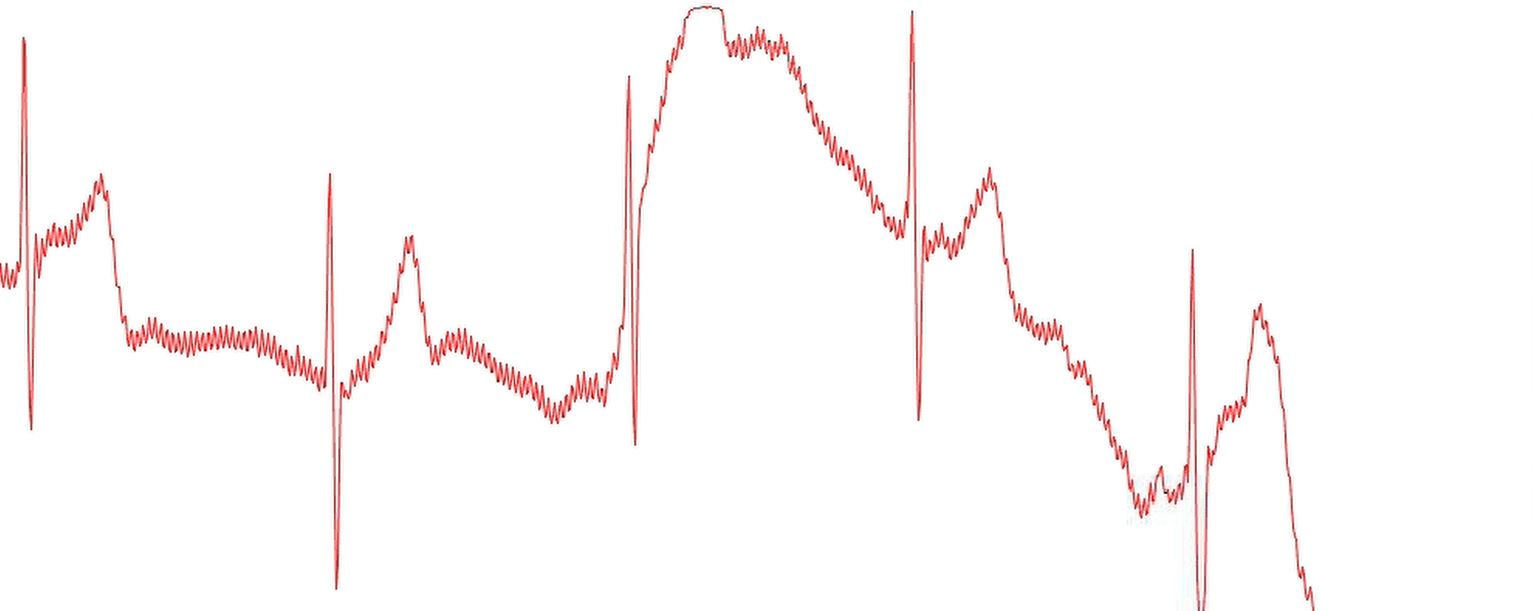
\includegraphics[width=\linewidth,height=40mm,frame]{ecgtest7.jpg}
	\caption{ECG Output with Limb Movement}
	\label{ecgmovement}
\end{figure} 

Inconsistent ECG readings are also caused by actual abnormalities or deficiencies in the heart but these cases are not discussed in this report as they are not relevant to the inherent sources of errors found in the ECG system. 


\section{Statistics}

SRW
	\chapter{Discussion}

\section{Challenges, Limitations, and Future Work}

The biggest challenge for this project is the time constraint introduced due to the delay in the necessary device delivery (12 weeks) and hence we could only focus on literature review and researching existing solutions. Development of hardware have only started in July, and there were some setbacks as the purchased sensors do not operate as expected and there have been difficulties in extracting vital information from those devices. 

Another setback was the diversity of sensors required in the project. EEG has been especially hard to develop, as medical standards EEG has strong amplifiers and advanced filters which we have not been able to replicate, rendering our EEG results to be non-satisfactory. This is also contributed by the lack of information from the selected chip manufacturer, which made the troubleshoot duration long and unproductive. 

Extensive research had been done in data prioritization protocols and programming but we were unable to integrate it into our systems due to the choice of virtual network computing in the end. This limits our capability to prioritize packet transmission via wireless as this will be done back-ended by the selected VNC server.  

The scope of the project is extremely broad, covering both the terminal and sensor design. Further in depth development and testing could be done if the sphere was narrowed down to either the design of the wireless terminal or specific sensors.  

\subsection{ECG}

The use of the AD8232 is a good decision due to the reliability of the IC. However, it is only good as a proof of concept and not for actual use in the medical industry as it does not meet regulatory standards. Another disadvantage of using the AD8232 is the use of only three electrodes rather than the usual 10-12 electrodes for standard ECG systems. 

It has been noticed that the output of the ECG has a moderately high frequency component which cannot be easily removed. This anomaly can be attributed to the frequency of the mains power supply. This chip was designed in the United States, where the mains power supply frequency is 60 Hz. Internally, the AD8232 has an inbuilt signal processing filter to remove this externally introduced noise. However, in Australia, the mains power supply frequency is set at 50 Hz. The ECG output is consistent with a small injection of power supply noise. To rectify this issue in future developments of this project, it is suggested to use either an electronic notch filter at 50 Hz or implement a signal processing filter at 50 Hz. This problem was only observed with the use of a connected power supply instead of a portable external battery. 

A PCB shield for the AD8232 and the Arduino Pro Mini was designed for this project. This PCB design can be found in Appendix \ref{ecgshieldpcb}. Nevertheless, it would be better to integrate the entire system onto a single board without the use of a shield. This was not done due to the broad scope of the project, leaving little time for other sections of the project if this aim was further pursued. 

The ECG is also an extremely sensitive component of the project, which provides differing results under similar circumstances. The results are not easy to replicate and extra care should be taken to ensure that testing conditions remain relatively the same, (i.e. the position and orientation of the patient). 

\subsection{EEG}
As EEG is easily affected by noise, a reliable front end will need to be devised. A notch filter will at 50Hz can be devised to filter of any noise that may be due to the power supply. This will be followed by a signal amplifier of approximately 10,000 gain to boost the measured 10 - 100uV to a measurable voltage of 100mV – 1V. Then, a low pass filter should be placed to filter of other noises from artifacts. 

The soldering of pins from EEG to the chip may also be a main contribution of why no reliable signal is detected in our application. This can be mitigated by purchasing a EEG head converter to pins rather than directly soldering the wire to the pads. The impurities in solder may cause the small signal to be gone prior to reaching the microchip, and hence the microchip will only detect noise during operation.

As EEG is relatively complex compared to the other parameters, it is suggested that a commercialized EEG amplifier to be used before we extract the information to be transmitted wirelessly. However, this have not been attempted due to the delay in delivery of sensors as well as budget constraints. 

\subsection{PPG}

The primary aim of this project is to demonstrate a working prototype system of wireless patient monitoring system. Since Raspberry Pi 3 Model B is chosen to be the Terminal of whole system and Arduino is used as an ADC for collecting analog signal, the remaining problem is how to connect a Pulse Oximeter to the Arduino and capture the desired signal. 

We started with the medical standard Pulse Oximeter (BioNomadix Wireless Wearable sensor) from Biopac Systems. The Pulse Oximeter is attached to a wireless transmitter module. Raw data are transferred via wireless communication to a receiver module and then to a wire connected PC. The signal processing and visualization is then performed on the PC. However, the BioNomadix Wireless system is fully developed commercial product such that we cannot get any access to either hardware or software. In another word, it is impossible to collect the PPG signal by connecting their Pulse Oximeter to our Raspberry Pi 3 model B. Hence, we decide to design our own Pulse Oximeter for proof of concept. We also believe that developing your own hardware is also a good practical experience.

Unfortunately, at this stage, the PPG we have designed is not able to detect the Oxygen Saturation level. However, a clean waveform and heart rate can be obtained from the sensor we designed. Oxygen Saturation level calculation is way more complicated than expected. 

Since this is a prototype designed mainly for collecting data for the wireless monitoring display, the current state of the waveform is sufficient for such a purpose. Calibration and noise cancellation can be implemented in the future to counter the issue such as signal variation due to the motion artifacts and noise from the power supply.

For this project, a PCB has been designed for the pulse oximeter. A simpler combination of integrated PCB with ADC and Pulse Oximeter can be used to replace the current design of connecting two separate pieces.

\subsection{Raspberry Pi}

\subsubsection{Power Efficiency}

According to Sohraby, Minoli, and Taieb \cite{sohraby2007wireless}, power efficiency can be achieved by having: 

\begin{enumerate}
	\item "Low-duty-cycle operation."
	\item "Local/in-network processing to reduce data volume (and hence transmission time)."
	\item "Multihop networking reduces the requirement for long-range transmission since signal path loss is an inverse exponent with range or distance. Each node in the sensor network can act as a repeater, thereby reducing the link range coverage required and, in turn, the transmission power." 
\end{enumerate}

\subsubsection{Security and Data Management}
The data measured via our system will be output in a readable format to be stored in the medical server for record purposes. This will be helpful when researchers/ health practitioners going through the surgical procedure to determine if anything was wrong. 

When disconnected due to unforeseen reasons, the buffer in the transmitter will record the information and re-transmits when connection resumed. A proposed solution would be cable available to link the transmission unit to a nearby monitor if the Local Area Network is down due to some unforeseen circumstances. 

\subsubsection{Reliability and Range}
As of the date of writing, Raspberry Pi has "uptime" of 81 days. This shows the reliability of the Raspberry Pi as a Terminal as it can operate for prolonged periods of time without freezing or crashing. 

\begin{lstlisting}
pi@raspberrypi:~/Desktop $ uptime
00:58:17 up 81 days, 23:21, 2 users, load average: 0.30, 0.19, 0.15
\end{lstlisting}

In terms of range, the Terminal has been tested to a range of up to 10m and has a throughput of 11.98Mbit/s \cite{wifibenchmark}. This is suitable for use in a moderately sized operating theatre. 

\subsubsection{Raspberry Pi Root USB}

Only a single root USB port is available on the Raspberry Pi 3 Model B and all data traffic from USB devices are directed to this single bus \cite{rpi3hardware}. The maximum speed of this root USB port is 480Mbps \cite{rpi3faqs}. The WVSMT utilises all 4 USB ports available for connections to individual Sensors and this could possibly lead to bottlenecking in the root USB port. However, it is noted that the bandwidth required for each sensor is low and that this scenario is not probable. 

\subsubsection{Consideration of Platform Upgrade}

One of the suggestions for the future development of this project is the replacement of the Raspberry Pi with a more powerful platform. The use of the Raspberry Pi is sufficient only as a proof of concept as it does not provide adequate processing power for further applications. Running concurrent processes such as VNC server hosting and data visualisation is possible but a small noticable lag is seen in the output waveform.   

A new platform can be designed from scratch but this would be very time consuming and requires technical expertise. Another option would be to consider upgrading the Raspberry Pi to an Intel NUC \cite{intelnuc}. The reason for not using such a platform from the start was due to cost constraints for prototyping. Now that the prototype is successfully working, it is highly recommended that a more powerful terminal be used in place of the Raspberry Pi.  
	\chapter{Conclusion }  
\label{Conclusion}

This report is result of the comprehensive documentation of the approach used and the design process of the wireless vital signs monitoring system. The development of the system encompasses two major sections, that is the Terminal design and the Sensor design. 

The Terminal chosen is the Raspberry Pi 3 Model B as it runs on a Linux-based OS, has WiFi capabilities, and has a sufficiently powerful processor for the purpose of this project. The Raspbian Jessie provides the needed kernel and OS foundation, allowing many needed applications to be installed and used. Data processing is done through Arduino, which converts a digital signal to a serial input. Data visualisation is completed in Processing 2.2.1, which plots real-time graphs of the vital signs monitored. Wireless data transmission is accomplished through the use of Tight VNC Server, which allows remote access from a separate Terminal, through the use of virtual network computing. This platform provides the foundation of the project as the main interface between the Sensors and display. 

The ECG sensor utilises the AD8232 IC from Analog Devices, which is a part of the front end for signal conditioning of the analog signal input received from the electrodes placed at specific locations on the skin surface. The amplified and filtered signal is then fed through an analog-to-digital converter and an FTDI-to-serial converter. The digital signal is then processed and visualised on the Terminal. The system has been tested successfully and shows a complete ECG output. 

The EEG sensor is comprised of the Neurosky TGAM module, which takes an input from electrodes placed on the surface of the scalp. It is a primary brainwave sensor ASIC module to process and output EEG frequency spectrum, EEG single quality, and raw EEG waveform. It has proved to be an extremely challenging part of the project due to the nature of the EEG signal amplitude. As such, it is suggested that a commercialized EEG amplifier to be used in future developments of this project. 

The PPG sensor utilises the GC1 PPG sensor, with an integrated infrared sensor, DC offset, high-pass filter, amplifier, and low-pass filter. The PPG sensor is fully capable of accurately capturing the SpO2 waveform and measuring the heart rate. The SpO2 concentration has been theoretically calculated and can be implemented in the future. 

The temperature sensor uses a simple thermistor in a phase shift oscillator configuration. This combination is suggested to make the frequency of the circuit temperature-dependent, mitigating the issue of self-heating in NTC thermistors, resulting in more accurate and reliable temperature readings. 

The diversity of this project is unique with a very broad scope, and each functional component has to be integrated together to function as a complete wireless vital signs monitoring system. It encompasses both front end development (sensors for data collection) and back end development (terminal for visualisation and wireless transmission). 

Overall, this project has generated sufficient evidence to show that the design of a wireless vital signs monitoring system for operating theatres is viable and feasible. The prototype constructed is a successful proof of concept, which paves the way for future development in the field of wireless medical systems.  
	
	\nocite{*}
	%\bibliographystyle{plain}
	\bibliographystyle{ieeetr}
	\bibliography{bibfile}	
	
	\appendix
	\chapter{Program Installation}

The operating system used for the project is Raspbian Jessie. To simplify installation, the SD card of the Raspberry Pi was flashed with an OS installer containing Raspbian Jessie, called NOOBS (New Out Of the Box Software) \cite{rpi3noobs}. When starting up, the loading screen will look typically like Figure \ref{rpi3noobs}. The version of NOOBS used was version 1.9.2, with a release date of 27/5/2016. 

\begin{figure}[H]
	\centering
	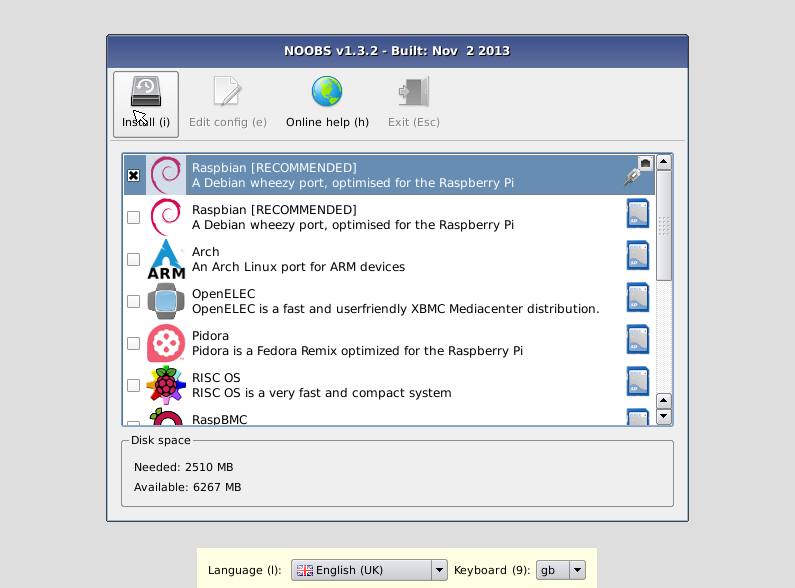
\includegraphics[width=\linewidth]{noobs.png}
	\caption{NOOBS (New Out Of the Box Software) Initial Installation Screen \cite{rpi3noobs}}
	\label{rpi3noobs}
\end{figure}

Aside from using NOOBS for the OS installation, it is possible to download the Raspbian Jessie image from the official Raspberry Pi website, unzip the image file, and copy it to the SD card. However, NOOBS was used specifically for its convenience, since it is necessary to obtain disk imager utilities on Windows for this method. Nevertheless, the choice of installation approach does not in any way affect the functionality of the OS after it has been loaded.  

\section{Operating System - Raspbian Jessie}
\label{appraspbianjessie}






\begin{lstlisting}
sudo apt-get update
sudo apt-get install tightvncserver
sudo apt-get install xtightvncviewer
sudo apt-get install arduino
sudo apt-get install python-matplotlib
\end{lstlisting}





\section{Code}

\subsection{Arduino Code for Thermistor}
\label{arduinothermistor}

\begin{lstlisting}[language=c]
/*
AnalogReadSerial
Reads an analog input on pin 0, prints the result to the serial monitor.
Attach the center pin of a potentiometer to pin A0, and the outside pins to +5V and ground.

This example code is in the public domain.
*/

#include <math.h>
#include <stdlib.h>
#include <stdio.h>

double T; 
double TK; 
double lnratio; 
double a, b, c, d; 

// the setup routine runs once when you press reset:
void setup() {
	// initialize serial communication at 9600 bits per second:
	Serial.begin(9600);
}

// the loop routine runs over and over again forever:
void loop() {
	// read the input on analog pin 0:
	double sensorValue = analogRead(A0);
	// print out the value you read:
	a = 3.3540154e-3;
	b = 2.5627725*pow(10,-4);
	c = 2.0829210*pow(10,-6);
	d = 7.3003206*pow(10,-8);
	
	// lnratio = log(sensorValue/(1023-sensorValue));
	for (double i=1;i<1024;i++) {
		lnratio = log(i/(1024-i));
		T = 1/(a+b*(lnratio)+c*pow(lnratio,2)+d*pow(lnratio,3)); 
		TK = T-273.15; 
		
		Serial.println(TK); 
		//Serial.print(' '); 
		//Serial.println(sensorValue);
		
		delay(1); 	// delay in between reads for stability
		}        
}
\end{lstlisting}

\subsection{Arduino Code for Phase Shift Oscillator}
\label{arduinopso}

\begin{lstlisting}[language=c]
#include <math.h>
double T = 0;  	/*Temperature*/
double t = 0;	/*Period*/
double F = 0;	/*Frequency*/

void setup() {

	/* Define pin 3 as an input */
	pinMode(3,INPUT);
	Serial.begin(9600); 
}

void loop() {

	while(digitalRead(3) == HIGH) {
	}; 
	while(digitalRead(3) == LOW) {
	};
	t = micros();
	while(digitalRead(3) == HIGH) {
	};
	while(digitalRead(3) == LOW) {
	}; 

	t = micros() - t;
	F = 1.0E6/t;
	T = 102.58*log(F) - 659.57; 

	Serial.println(T); 
	delay(1); 
}

\end{lstlisting}

\subsection{MATLAB ECG Simulation}
\label{ecgsimulationcode}

The simulated ECG signal in Figure \ref{ecgsim} in Section \ref{simulation} was obtained by running the following code in MATLAB.

\begin{lstlisting}
>>ECGwaveGen(70,5,500,2500)
\end{lstlisting}

The ECGwaveGen.m file below was obtained from physionet.org \cite{ecgsimulation}.

\begin{lstlisting}[language=Matlab]
function [QRSwave]=ECGwaveGen(bpm,duration,fs,amp)
%[QRSwave]=ECGwaveGen(bpm,dur,fs,amp) generates an artificial ECG/EKG waveform
%    Heart rate (bpm) sets the qrs event frequency (RR interval). 
%    Duration of the entire waveform (dur) is in units of seconds.
%    Sample frequency (fs) sets the sample frequency in Hertz. 
%    Amplitude (amp) of the QRS event is measured in micro Volts. The
%    waveform consists of a QRS complex and a T-wave. No attempt to 
%    represent a P-wave has been made.
%     
%    There are two additional parameters that can be changed from within the function.
%    They are the parameters that set the QRS width (default 0.1 secs) and the t-wave 
%    amplitude (default 500 uV).

%Created January 22, 2001 by Floyd Harriott, primary email (fharriott@stellate.com), secondary email (fsh@po.cwru.edu)
%Modified March 19, 2002 by Floyd Harriott, extended default duration so that default settings produce a QRS event rather than 
%   an error. Allows for the random insertion of PVCs.  This file must be edited to include PVCs.

%Algorithm is based in part on the jounal article:
%Ruha, Antti and Seppo Nissila, "A Real-Time Microprocessor QRS Detector System with a 1-ms Timing Accuracy
%      for the Measurement of Ambulatory HRV", IEEE Trans. Biomed. Eng. Vol. 44, No. 3, 1997
%The artificial ECG signal they describe is based on the recommendations in the Association for the Advancement
%of Medical Instrumentation (AAMI) "Standard for Cardiac Monitors, Heart Rate Meters and Alarms (draft), Aug. 1981
%Feel free to make modifications, corrections and or suggestions.

if (exist('fs') ~= 1)  fs=  200;   end  %default value, Hz
if (exist('bpm') ~= 1)  bpm =  72;   end %default value, beats per minute
if (exist('amp') ~= 1)  amp = 1000;   end %default value, micro volts
if (exist('duration') ~= 1)  duration =  (60/bpm-0.35)+60/bpm+1/fs; end  %default value gives one cycle, seconds

global t_line; %seconds
global sample_freq; % always equal to fs


%Changeable Parameters
d=0.1; %.07 to .120 seconds, QRS width
at=500; %amplitude of t-wave, 400 to 1200 uv

%Should not touch
org_amp=amp;
sample_freq=fs; %duplicated simply to make a global version
RR=(60/bpm); %RR interval, seconds
d1=0.4375*d;
d2=0.5*d;
d3=d-(d1+d2);
dt=0.180; %width of t wave, seconds
qt=0.35; %time from beginning of QRS to end of t-wave
t_line=0:1/fs:duration; %time line, seconds
QRS_wave=zeros( size(t_line) ); %QRS waveform
deadspace=RR-qt; %time between t-wave and next QRS
if deadspace < 0 
err_msg=['Bpm must be equal to or less than ' int2str(60/qt) ' inorder to fit one cycle.'];
error(err_msg); 
end


%Calculate PVC parameters and segment
PVCchance=0.1; %How often does PVC happen., percent eg. 0.1=10%
PVCamp=amp;    %PVC amplitude, eg. same as normals (amp)
earlyfactor=0.25; %percentage, how much early should PVC happen then normal RR interval
PVCwidth=0.12; %seconds, QRS width of PVC, usually .12 to .17
PVCseg=[QRSpulse(d,60/((1-earlyfactor)*RR-0.4375*PVCwidth),fs,RandAmp(org_amp)) QRSpulse(PVCwidth,bpm*(1-earlyfactor),fs,PVCamp) QRSpulse(d,bpm,fs, RandAmp(org_amp))]; %PVC segment
tPVC=size(PVCseg,2)/fs; %amount of time taken up by PVC segment in seconds

t1=deadspace; %Where does the first QRS start? eg deadspace, or 0

%need enough time to display at least one interval.
if (t1+60/bpm+1/sample_freq > duration)
err_msg=['The waveform length (duration) must be more than ' sprintf('%.2f%',t1+60/bpm+1/sample_freq) ' second(s) in order to display one QRS event.'];
error(err_msg);
end


%GENERATION LOOP
while ( t1+60/bpm+1/sample_freq <= duration) %space to insert another qrs pulse in time line

%amp=RandAmp(org_amp); %random size on qrs event
amp=org_amp;



%Segment 1  (Q-R)
qrs_start=t1;   
t2=t1+d1;
i_t1=time2index(t1); i_t2=time2index(t2);
left=0; right=0.875*amp;
m1=(right-left)/(t2-t1);
QRS1=m1*index2time(i_t1:i_t2)-(m1*t1-left);
QRSwave(i_t1:i_t2)=QRS1;

%Segment 2  (R-?)
t1=t2; t2=t1+d2;
i_t1=time2index(t1); i_t2=time2index(t2);
left=right; right=-.125*amp;
m2=(right-left)/(t2-t1);
QRS1=m2*index2time(i_t1:i_t2)-(m2*t1-left);
QRSwave(i_t1:i_t2)=QRS1;


%Segment 3 bottom_top (?-S) 
t1=t2; t2=t1+d3; 
i_t1=time2index(t1); i_t2=time2index(t2);
left=right; right=0;
if (i_t2-i_t1 >0) %at low sampling freq. there may be no sample for this segment
m3=(right-left)/(t2-t1);
QRS1=m3*index2time(i_t1:i_t2)-(m3*t1-left);
QRS1=QRS1( find(QRS1<=0));
QRSwave(i_t1:i_t1+size(QRS1,2)-1)=QRS1;
elseif i_t2-i_t1==0
m3=(right-left)/(t2-t1);
QRS1=m3*index2time(i_t1:i_t2)-(m3*t1-left);
QRSwave(i_t1)=QRS1(1);
end

%Segment 4, S-T interval
t1=t2; t2=t1+qt+qrs_start-(dt+t2);
i_t1=time2index(t1); i_t2=time2index(t2);
left=right; right=0;

%Segment 5, t-wave
t1=t2; t2=t1+dt;
i_t1=time2index(t1); i_t2=time2index(t2);
t=-1:2/(i_t2-i_t1):1;
QRS1=at*sqrt(1-t.^2);
QRSwave(i_t1:i_t2)=QRS1;

%Segment 6, remaining deadspace
t1=t2; t2=t1+deadspace;
i_t1=time2index(t1); i_t2=time2index(t2);


%Do we insert a PVC here? Roll the die and find out.
insertPVC=rand(1); %uncomment following 5 lines if PVCs are desired.
%if insertPVC<=PVCchance & t2+tPVC+2/sample_freq <= duration %enough space to insert PVC
%   t1=t2; t2=t1+tPVC;
%  i_t1=time2index(t1); i_t2=time2index(t2);
% QRSwave(i_t1:i_t1+size(PVCseg,2)-1)=PVCseg;
%end

%stem(QRSwave); % view ECG waveform
t1=t2; %end of this segment becomes beginning of next segment

end %while loop, appending qrs pulses

%_____________________________________%
function index=time2index(t)
%TIME2INDEX converts time (s) to an index value

global t_line;

indexArray=find(t_line>=t);
index=indexArray(1); 

%_____________________________________%
function time=index2time(i)
%INDEX2TIME converts a time line index to a time value (seconds)
global sample_freq

time=(i-1).*1/sample_freq;


%_____________________________________%
function RAmp=RandAmp(orgAmp)

RAmp=orgAmp+0.4*orgAmp*rand(1);
\end{lstlisting}

	\chapter{PCB Design and Schematics}

SEPARATE DESIGN AND SCHEMATICS

\section{ECG Shield for AD8232 and Arduino Pro Mini}
\label{ecgshieldpcb}

\section{Blood Temperature}

\section{AD8232 Heart Rate Monitor SparkFun Implementation}

\begin{figure}[H]
	\centering
	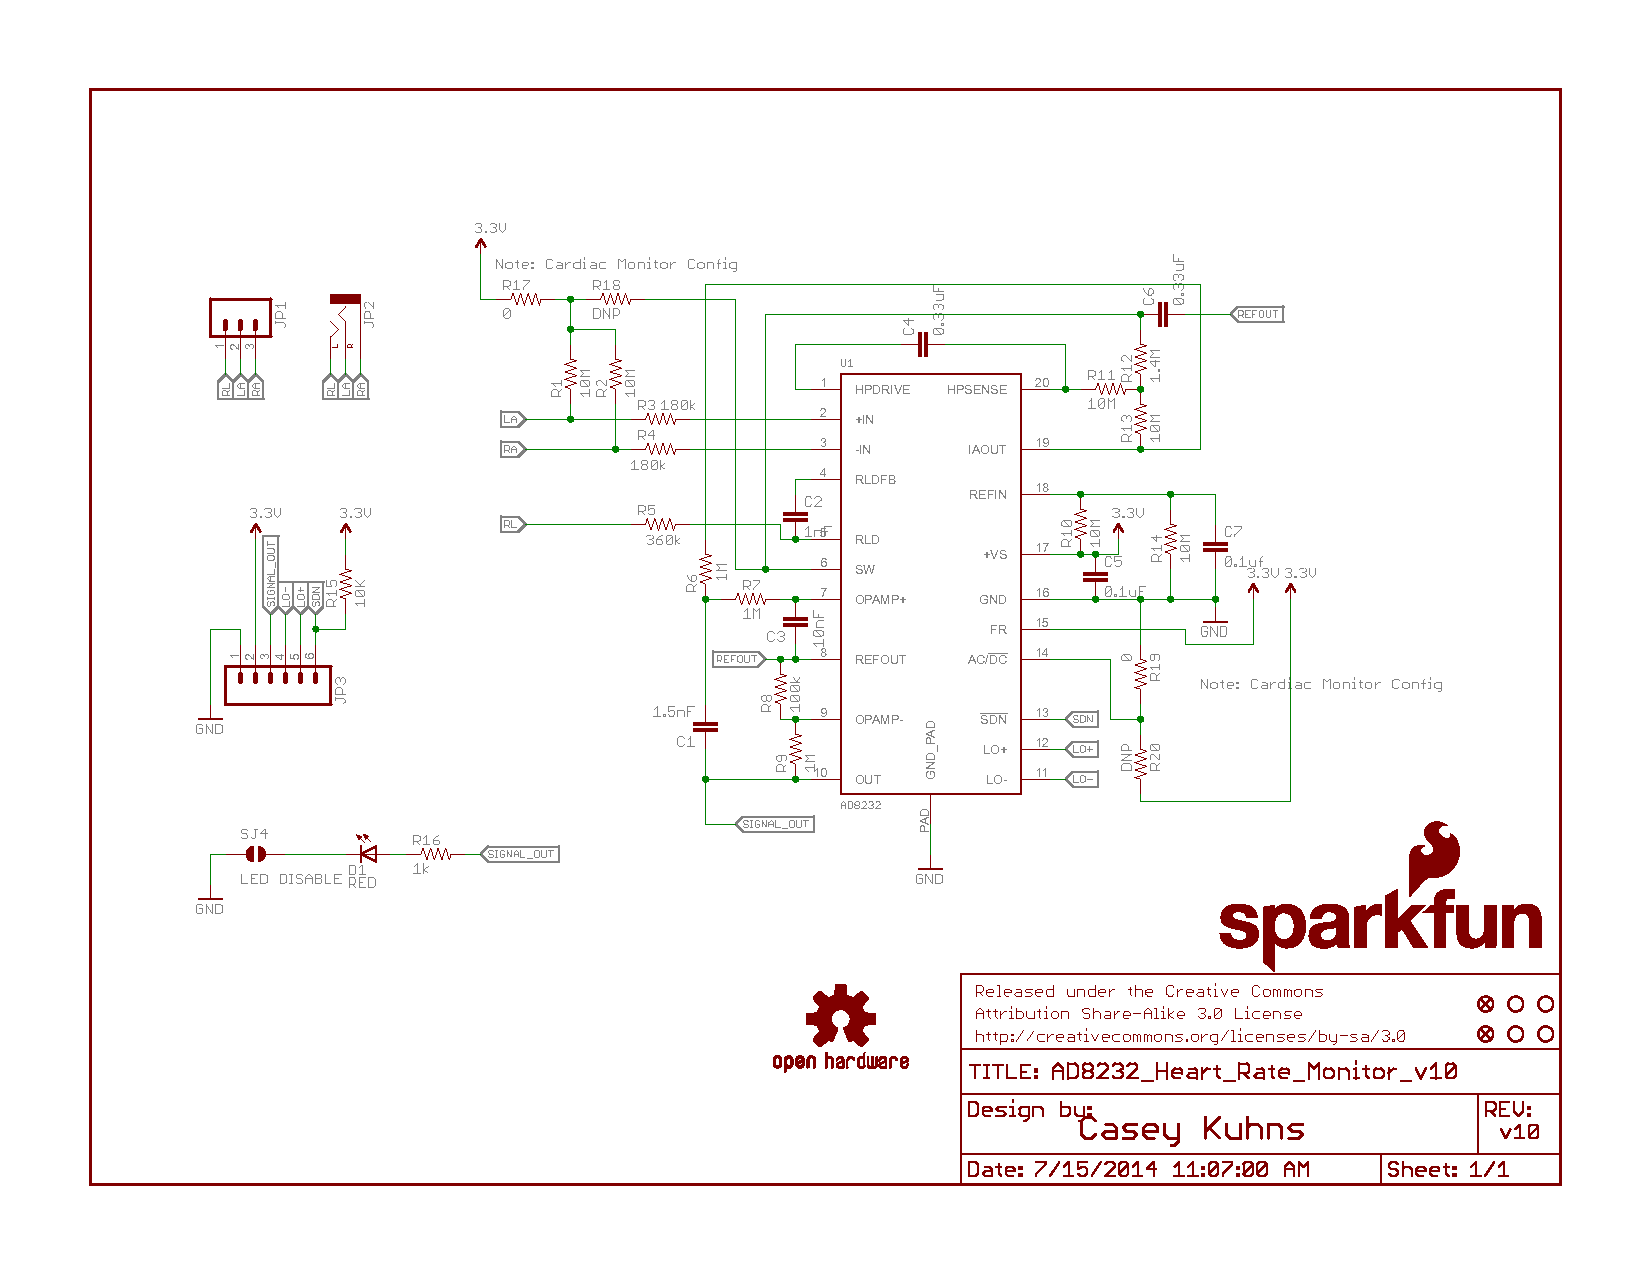
\includegraphics[width=1.05\linewidth]{AD8232_Heart_Rate_Monitor_v10.pdf}
	\caption{AD8232 SparkFun Implementation Schematic Diagram \cite{ad8232sfschematic}}
	\label{ad8232sfschematic}
\end{figure}

Further details of the design can be found at \\ https://github.com/sparkfun/AD8232\_Heart\_Rate\_Monitor.

\section{Raspberry Pi 3 Model B}

\begin{figure}[H]
	\centering
	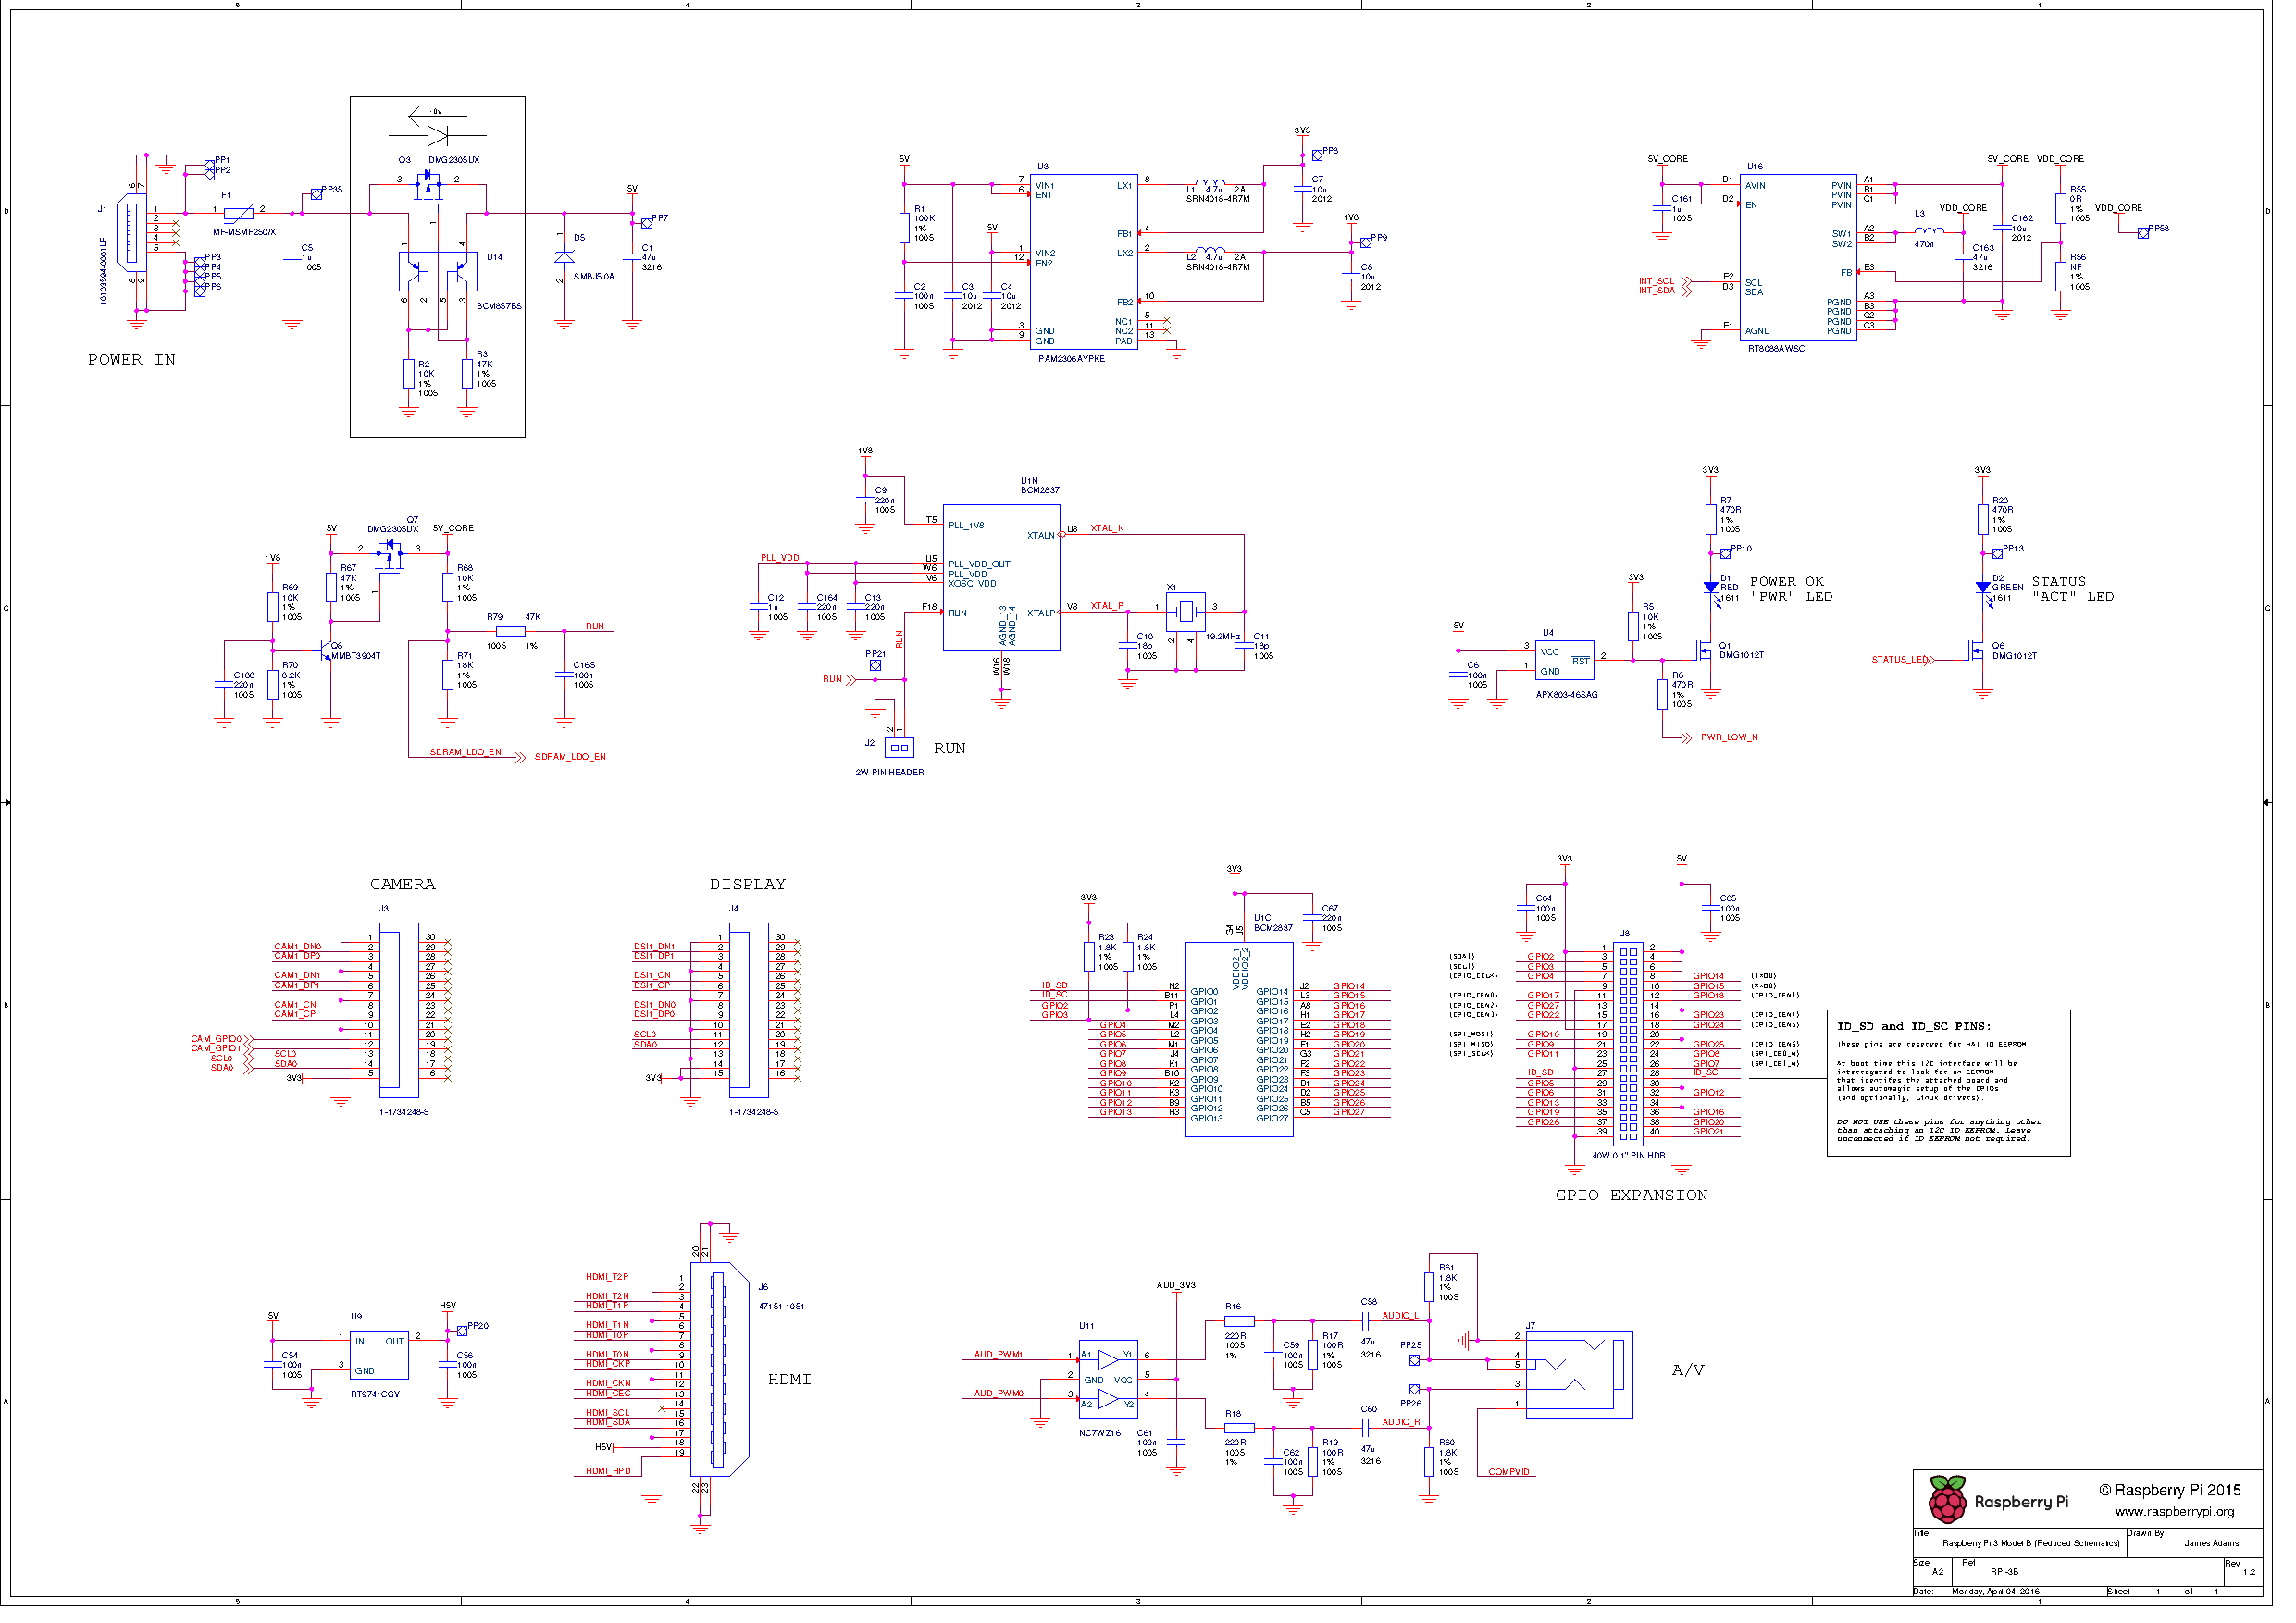
\includegraphics[width=1.25\linewidth,angle=90,origin=c]{RPI-3B.pdf}
	\caption{Raspberry Pi 3 Model B Schematic Diagram \cite{rpi3hardware}}
	\label{rpi3bschematic}
\end{figure}

Further details of the design can be found at \\ https://www.raspberrypi.org/documentation/hardware/raspberrypi/schematics/RPI-3B-V1\_2-SCHEMATIC-REDUCED.pdf.
	\input{appendixpower.tex}
	\chapter{Measurements and Datasheets} 

\section{Datasheet}

\begin{figure}[H]
	\centering
	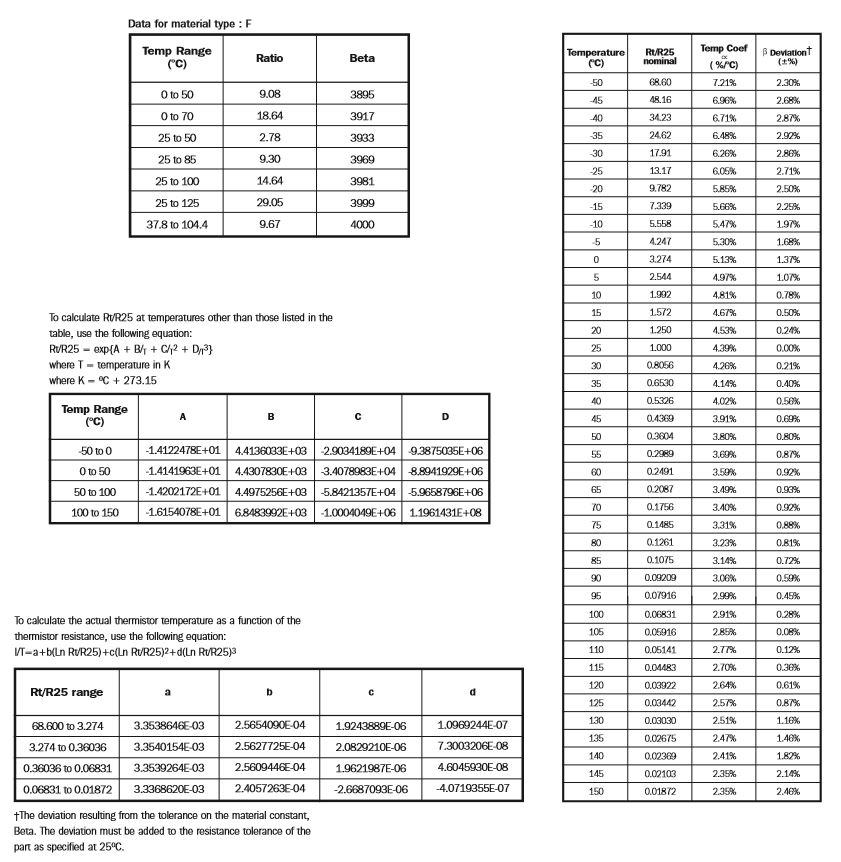
\includegraphics[width=0.8\linewidth]{thermistordatasheet.jpg}
	\caption{Snippet of Material Type F Thermistor Datasheet \cite{thermistor}}
	\label{thermistordatasheet}
\end{figure}

By plotting Equation \ref{thermistorresistance1} throughout the temperature range, we obtain Figure \ref{RTR25temperature}. 

\begin{figure}[H]
	\centering
	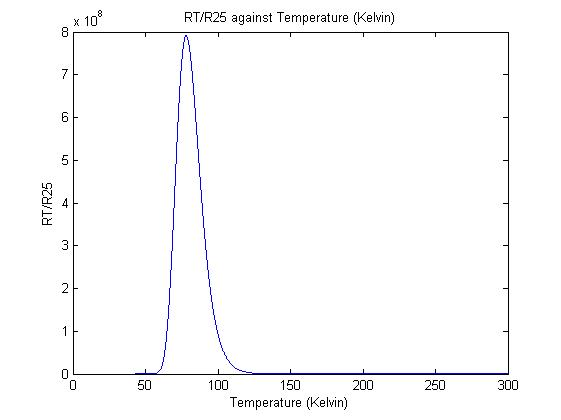
\includegraphics[width=0.8\linewidth]{thermistor4.jpg}
	\caption{RT/R25 against Temperature (Kelvin)}
	\label{RTR25temperature}
\end{figure}

\section{Summary of Output Frequency, R1 Resistance, and Temperature}
\label{appthermistorpso}

\begin{table}[H]
	\centering
	\begin{tabular}{|l|l|l|}
		\hline
		\textbf{Frequency (Average) (Hz)} & \textbf{Resistor (k ohm)} & \textbf{Temperature ($\degree C$)} \\ \hline
		713.84                  & 16                        & 14.62522155              \\ \hline
		793.2                   & 10                        & 25.00009198              \\ \hline
		759.49                  & 12                        & 20.89759901              \\ \hline
		668.81                  & 23                        & 7.043807812              \\ \hline
		810.8                   & 9                         & 27.41774841              \\ \hline
		657.95                  & 25                        & 5.351508212              \\ \hline
		868.13                  & 6.7                       & 34.38035887              \\ \hline
		667.96                  & 22                        & 7.953407074              \\ \hline
		746.29                  & 13                        & 19.12817814              \\ \hline
		1008.56                 & 3.6                       & 50.02636632              \\ \hline
		712.37                  & 16                        & 14.62522155              \\ \hline
		694.47                  & 18                        & 12.12527069              \\ \hline
		885.42                  & 6.2                       & 36.2584574               \\ \hline
		810.08                  & 9                         & 27.41774841              \\ \hline
		848.1                   & 7.5                       & 31.68532759              \\ \hline
		695.69                  & 18                        & 12.12527069              \\ \hline
		694.83                  & 18                        & 12.12527069              \\ \hline
		668.5                   & 22                        & 7.953407074              \\ \hline
		984.74                  & 3.9                       & 47.93002289              \\ \hline
	\end{tabular}
	\caption{Summary of Output Frequency, $R_1$ Resistance, and Temperature}
	\label{psocalibrationsummary}
\end{table}

\section{Phase Shift Oscillator Calibration}
\label{psocalibration}

For the calibration of the phase shift oscillator frequency for specific resistances of the thermistor, the output frequency measured by the Arduino Uno is recorded as found in Tables \ref{calibrationtable1}, \ref{calibrationtable2}, and \ref{calibrationtable3} below for each resistor value chosen. This process is repeated 100 times for each resistor to find the average output frequency corresponding to that resistance of $R_1$.  \\

\subsection{Astable Operation of 555 Timer}

Another method of signal condition for the thermistor involves using the 555 Timer in astable operation. 

555 Timer Datasheet. 

\subsection{Priority Queueing Models}

As in our proposed model, there will be multiple sensors, namely EEG, ECG, PPG etc. that are integrated into one transmission, a priority queueing model will need to be devised to ensure important vital signs data are prioritized when bandwidth / throughput is limited at certain stages of transmission. An appropriate queuing models are implemented to improve performance parameters for priority queueing, delay and server utilization time. In a study conducted by The NorthCap University \cite{lit4} indicate that using M/G/1 Or M/G/N queueing models will have better performance depending on the expected number of incoming packets. An extract of the results is shown below, serving as a reference to our queueing model. 

\begin{figure}[H]
	\centering
	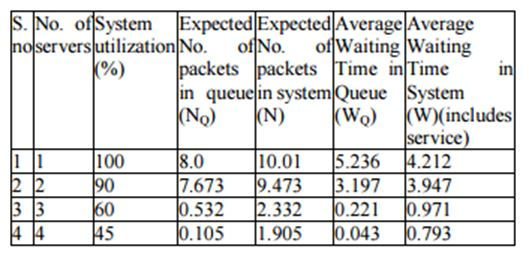
\includegraphics[width=0.5\linewidth]{lit3.jpg}
	\caption{Result for M/G/1 and M/G/N queueing models for the proposed scenario \cite{lit4}}
	\label{literaturereview3}
\end{figure}



	\begin{longtable}{|l|l|l|l|l|l|l|l|l|}

		\hline
		16 k ohm & 10k ohm & 12k ohm & 23k ohm & 9k ohm & 25k ohm & 6.7k ohm & 22k ohm & 13k ohm \\ \hline
		714.29   & 791.14  & 757.58  & 666.67  & 811.69 & 656.17  & 868.06   & 672.04  & 744.05  \\ \hline
		712.25   & 793.65  & 757.58  & 670.24  & 809.06 & 659.63  & 874.13   & 664.89  & 753.01  \\ \hline
		716.33   & 791.14  & 759.88  & 670.24  & 809.06 & 656.17  & 856.16   & 664.89  & 744.05  \\ \hline
		714.29   & 791.14  & 762.2   & 668.45  & 811.69 & 656.17  & 862.07   & 672.04  & 744.05  \\ \hline
		712.25   & 796.18  & 759.88  & 670.24  & 806.45 & 657.89  & 868.06   & 672.04  & 744.05  \\ \hline
		714.29   & 791.14  & 759.88  & 668.45  & 809.06 & 659.63  & 868.06   & 672.04  & 753.01  \\ \hline
		712.25   & 793.65  & 757.58  & 666.67  & 811.69 & 659.63  & 868.06   & 664.89  & 744.05  \\ \hline
		716.33   & 793.65  & 762.2   & 670.24  & 811.69 & 656.17  & 868.06   & 672.04  & 744.05  \\ \hline
		716.33   & 793.65  & 759.88  & 670.24  & 811.69 & 657.89  & 868.06   & 672.04  & 744.05  \\ \hline
		714.29   & 791.14  & 762.2   & 668.45  & 809.06 & 656.17  & 868.06   & 672.04  & 744.05  \\ \hline
		716.33   & 793.65  & 757.58  & 670.24  & 811.69 & 657.89  & 868.06   & 672.04  & 744.05  \\ \hline
		712.25   & 791.14  & 759.88  & 668.45  & 816.99 & 657.89  & 874.13   & 664.89  & 753.01  \\ \hline
		714.29   & 793.65  & 757.58  & 668.45  & 811.69 & 656.17  & 874.13   & 672.04  & 744.05  \\ \hline
		714.29   & 793.65  & 757.58  & 668.45  & 811.69 & 657.89  & 868.06   & 664.89  & 744.05  \\ \hline
		714.29   & 791.14  & 757.58  & 668.45  & 811.69 & 657.89  & 868.06   & 672.04  & 753.01  \\ \hline
		714.29   & 793.65  & 757.58  & 666.67  & 809.06 & 656.17  & 868.06   & 672.04  & 744.05  \\ \hline
		714.29   & 793.65  & 757.58  & 666.67  & 811.69 & 659.63  & 868.06   & 664.89  & 744.05  \\ \hline
		716.33   & 793.65  & 762.2   & 666.67  & 811.69 & 657.89  & 868.06   & 664.89  & 744.05  \\ \hline
		714.29   & 793.65  & 757.58  & 666.67  & 811.69 & 656.17  & 868.06   & 664.89  & 753.01  \\ \hline
		714.29   & 793.65  & 759.88  & 668.45  & 811.69 & 656.17  & 868.06   & 672.04  & 753.01  \\ \hline
		714.29   & 793.65  & 759.88  & 670.24  & 811.69 & 657.89  & 868.06   & 664.89  & 753.01  \\ \hline
		712.25   & 793.65  & 757.58  & 668.45  & 811.69 & 657.89  & 874.13   & 664.89  & 753.01  \\ \hline
		716.33   & 793.65  & 759.88  & 670.24  & 811.69 & 656.17  & 862.07   & 672.04  & 753.01  \\ \hline
		714.29   & 793.65  & 759.88  & 670.24  & 811.69 & 656.17  & 856.16   & 672.04  & 744.05  \\ \hline
		712.25   & 793.65  & 757.58  & 668.45  & 811.69 & 657.89  & 868.06   & 672.04  & 744.05  \\ \hline
		714.29   & 791.14  & 757.58  & 670.24  & 811.69 & 657.89  & 868.06   & 664.89  & 744.05  \\ \hline
		714.29   & 791.14  & 759.88  & 670.24  & 811.69 & 659.63  & 868.06   & 672.04  & 744.05  \\ \hline
		712.25   & 791.14  & 759.88  & 668.45  & 809.06 & 656.17  & 868.06   & 672.04  & 744.05  \\ \hline
		712.25   & 793.65  & 759.88  & 670.24  & 811.69 & 657.89  & 874.13   & 664.89  & 744.05  \\ \hline
		712.25   & 793.65  & 759.88  & 670.24  & 811.69 & 657.89  & 868.06   & 664.89  & 744.05  \\ \hline
		712.25   & 793.65  & 759.88  & 668.45  & 806.45 & 657.89  & 868.06   & 664.89  & 753.01  \\ \hline
		714.29   & 796.18  & 759.88  & 670.24  & 811.69 & 657.89  & 868.06   & 672.04  & 744.05  \\ \hline
		712.25   & 793.65  & 762.2   & 668.45  & 811.69 & 656.17  & 874.13   & 664.89  & 753.01  \\ \hline
		714.29   & 791.14  & 759.88  & 668.45  & 809.06 & 659.63  & 868.06   & 664.89  & 744.05  \\ \hline
		714.29   & 791.14  & 757.58  & 666.67  & 811.69 & 656.17  & 868.06   & 664.89  & 744.05  \\ \hline
		714.29   & 793.65  & 759.88  & 668.45  & 811.69 & 656.17  & 868.06   & 672.04  & 744.05  \\ \hline
		716.33   & 793.65  & 759.88  & 670.24  & 811.69 & 659.63  & 868.06   & 672.04  & 753.01  \\ \hline
		712.25   & 793.65  & 759.88  & 668.45  & 811.69 & 657.89  & 868.06   & 664.89  & 744.05  \\ \hline
		712.25   & 791.14  & 757.58  & 670.24  & 811.69 & 659.63  & 868.06   & 664.89  & 744.05  \\ \hline
		712.25   & 793.65  & 757.58  & 668.45  & 809.06 & 656.17  & 868.06   & 672.04  & 753.01  \\ \hline
		716.33   & 793.65  & 759.88  & 670.24  & 809.06 & 657.89  & 868.06   & 664.89  & 744.05  \\ \hline
		712.25   & 796.18  & 757.58  & 670.24  & 809.06 & 659.63  & 868.06   & 672.04  & 744.05  \\ \hline
		712.25   & 793.65  & 757.58  & 668.45  & 811.69 & 657.89  & 868.06   & 672.04  & 744.05  \\ \hline
		716.33   & 793.65  & 757.58  & 670.24  & 809.06 & 656.17  & 868.06   & 664.89  & 744.05  \\ \hline
		712.25   & 791.14  & 759.88  & 670.24  & 803.86 & 657.89  & 868.06   & 664.89  & 744.05  \\ \hline
		714.29   & 793.65  & 762.2   & 666.67  & 811.69 & 659.63  & 868.06   & 664.89  & 753.01  \\ \hline
		712.25   & 791.14  & 759.88  & 666.67  & 809.06 & 657.89  & 868.06   & 664.89  & 744.05  \\ \hline
		714.29   & 793.65  & 757.58  & 668.45  & 811.69 & 656.17  & 874.13   & 664.89  & 744.05  \\ \hline
		716.33   & 793.65  & 757.58  & 668.45  & 811.69 & 657.89  & 868.06   & 664.89  & 744.05  \\ \hline
		712.25   & 793.65  & 762.2   & 668.45  & 806.45 & 654.45  & 868.06   & 664.89  & 744.05  \\ \hline
		712.25   & 793.65  & 759.88  & 668.45  & 811.69 & 657.89  & 868.06   & 672.04  & 744.05  \\ \hline
		714.29   & 793.65  & 757.58  & 668.45  & 811.69 & 657.89  & 874.13   & 672.04  & 744.05  \\ \hline
		712.25   & 793.65  & 757.58  & 670.24  & 811.69 & 657.89  & 868.06   & 672.04  & 744.05  \\ \hline
		714.29   & 793.65  & 759.88  & 666.67  & 811.69 & 657.89  & 868.06   & 672.04  & 753.01  \\ \hline
		714.29   & 793.65  & 757.58  & 668.45  & 811.69 & 659.63  & 868.06   & 672.04  & 744.05  \\ \hline
		712.25   & 793.65  & 757.58  & 668.45  & 811.69 & 659.63  & 868.06   & 664.89  & 744.05  \\ \hline
		714.29   & 793.65  & 757.58  & 670.24  & 809.06 & 657.89  & 868.06   & 672.04  & 753.01  \\ \hline
		712.25   & 796.18  & 759.88  & 668.45  & 811.69 & 657.89  & 868.06   & 664.89  & 744.05  \\ \hline
		712.25   & 793.65  & 759.88  & 668.45  & 811.69 & 657.89  & 868.06   & 672.04  & 753.01  \\ \hline
		714.29   & 796.18  & 757.58  & 668.45  & 809.06 & 656.17  & 868.06   & 664.89  & 744.05  \\ \hline
		712.25   & 793.65  & 757.58  & 668.45  & 809.06 & 656.17  & 868.06   & 672.04  & 753.01  \\ \hline
		712.25   & 793.65  & 762.2   & 668.45  & 811.69 & 656.17  & 868.06   & 672.04  & 744.05  \\ \hline
		714.29   & 793.65  & 757.58  & 670.24  & 811.69 & 656.17  & 868.06   & 664.89  & 744.05  \\ \hline
		714.29   & 793.65  & 762.2   & 670.24  & 814.33 & 659.63  & 868.06   & 664.89  & 753.01  \\ \hline
		716.33   & 793.65  & 762.2   & 670.24  & 809.06 & 659.63  & 868.06   & 664.89  & 744.05  \\ \hline
		714.29   & 793.65  & 759.88  & 670.24  & 809.06 & 659.63  & 868.06   & 664.89  & 744.05  \\ \hline
		714.29   & 793.65  & 759.88  & 668.45  & 811.69 & 656.17  & 868.06   & 672.04  & 744.05  \\ \hline
		714.29   & 796.18  & 759.88  & 670.24  & 811.69 & 656.17  & 868.06   & 672.04  & 744.05  \\ \hline
		712.25   & 793.65  & 757.58  & 666.67  & 809.06 & 657.89  & 868.06   & 664.89  & 753.01  \\ \hline
		712.25   & 791.14  & 762.2   & 666.67  & 811.69 & 657.89  & 868.06   & 672.04  & 744.05  \\ \hline
		714.29   & 793.65  & 757.58  & 670.24  & 809.06 & 656.17  & 868.06   & 664.89  & 744.05  \\ \hline
		712.25   & 793.65  & 759.88  & 666.67  & 811.69 & 657.89  & 868.06   & 664.89  & 744.05  \\ \hline
		714.29   & 793.65  & 759.88  & 670.24  & 809.06 & 661.38  & 868.06   & 664.89  & 744.05  \\ \hline
		714.29   & 793.65  & 759.88  & 668.45  & 809.06 & 657.89  & 868.06   & 664.89  & 744.05  \\ \hline
		714.29   & 793.65  & 759.88  & 670.24  & 811.69 & 659.63  & 868.06   & 664.89  & 744.05  \\ \hline
		712.25   & 793.65  & 759.88  & 666.67  & 811.69 & 657.89  & 868.06   & 664.89  & 744.05  \\ \hline
		712.25   & 793.65  & 759.88  & 668.45  & 811.69 & 661.38  & 868.06   & 664.89  & 744.05  \\ \hline
		712.25   & 793.65  & 757.58  & 666.67  & 811.69 & 656.17  & 868.06   & 664.89  & 744.05  \\ \hline
		710.23   & 791.14  & 759.88  & 668.45  & 809.06 & 661.38  & 868.06   & 664.89  & 744.05  \\ \hline
		714.29   & 793.65  & 762.2   & 666.67  & 811.69 & 659.63  & 868.06   & 664.89  & 744.05  \\ \hline
		714.29   & 788.64  & 759.88  & 668.45  & 811.69 & 661.38  & 868.06   & 664.89  & 744.05  \\ \hline
		712.25   & 793.65  & 759.88  & 668.45  & 809.06 & 657.89  & 868.06   & 664.89  & 753.01  \\ \hline
		712.25   & 793.65  & 757.58  & 668.45  & 811.69 & 661.38  & 868.06   & 672.04  & 753.01  \\ \hline
		712.25   & 793.65  & 757.58  & 670.24  & 811.69 & 659.63  & 868.06   & 672.04  & 753.01  \\ \hline
		714.29   & 793.65  & 759.88  & 670.24  & 811.69 & 657.89  & 862.07   & 664.89  & 744.05  \\ \hline
		714.29   & 793.65  & 757.58  & 672.04  & 809.06 & 657.89  & 868.06   & 672.04  & 744.05  \\ \hline
		712.25   & 791.14  & 759.88  & 668.45  & 811.69 & 659.63  & 862.07   & 672.04  & 744.05  \\ \hline
		714.29   & 793.65  & 759.88  & 666.67  & 811.69 & 659.63  & 874.13   & 664.89  & 744.05  \\ \hline
		716.33   & 791.14  & 764.53  & 670.24  & 809.06 & 659.63  & 868.06   & 664.89  & 744.05  \\ \hline
		716.33   & 791.14  & 762.2   & 668.45  & 814.33 & 656.17  & 868.06   & 672.04  & 744.05  \\ \hline
		714.29   & 791.14  & 759.88  & 666.67  & 806.45 & 661.38  & 868.06   & 672.04  & 744.05  \\ \hline
		712.25   & 793.65  & 759.88  & 668.45  & 811.69 & 656.17  & 868.06   & 672.04  & 744.05  \\ \hline
		716.33   & 793.65  & 757.58  & 670.24  & 811.69 & 659.63  & 868.06   & 664.89  & 744.05  \\ \hline
		714.29   & 793.65  & 759.88  & 670.24  & 811.69 & 657.89  & 868.06   & 664.89  & 744.05  \\ \hline
		714.29   & 793.65  & 764.53  & 666.67  & 806.45 & 657.89  & 868.06   & 664.89  & 744.05  \\ \hline
		716.33   & 793.65  & 762.2   & 670.24  & 811.69 & 656.17  & 868.06   & 672.04  & 744.05  \\ \hline
		718.39   & 791.14  & 762.2   & 666.67  & 811.69 & 659.63  & 868.06   & 664.89  & 744.05  \\ \hline
		714.29   & 793.65  & 762.2   & 670.24  & 811.69 & 657.89  & 868.06   & 664.89  & 753.01  \\ \hline
		714.29   & 793.65  & 759.88  & 670.24  & 811.69 & 657.89  & 868.06   & 664.89  & 744.05  \\ \hline
		714.29   & 793.65  & 757.58  & 668.45  & 811.69 & 656.17  & 868.06   & 664.89  & 753.01  \\ \hline
		\caption{Output Frequency based on R1 Values}		\label{calibrationtable1}
	\end{longtable}
	
	
	

\begin{longtable}{|l|l|l|l|l|l|l|l|l|l|}
		\hline
		3.6k ohm & 16k ohm & 18k ohm & 6.2k ohm & 9k ohm & 7.5k ohm & 18k ohm & 18k ohm & 22k ohm \\ \hline
		1041.67  & 710.23  & 694.44  & 868.06   & 809.06 & 850.34   & 694.44  & 694.44  & 670.24  \\ \hline
		1008.06  & 710.23  & 694.44  & 919.12   & 806.45 & 844.59   & 694.44  & 694.44  & 666.67  \\ \hline
		1008.06  & 710.23  & 694.44  & 919.12   & 811.69 & 844.59   & 694.44  & 694.44  & 668.45  \\ \hline
		1008.06  & 710.23  & 694.44  & 868.06   & 811.69 & 844.59   & 702.25  & 694.44  & 666.67  \\ \hline
		1008.06  & 726.74  & 694.44  & 919.12   & 809.06 & 844.59   & 694.44  & 694.44  & 670.24  \\ \hline
		1008.06  & 710.23  & 679.35  & 919.12   & 811.69 & 850.34   & 694.44  & 694.44  & 668.45  \\ \hline
		1041.67  & 710.23  & 694.44  & 868.06   & 809.06 & 844.59   & 694.44  & 694.44  & 670.24  \\ \hline
		976.56   & 710.23  & 694.44  & 868.06   & 811.69 & 850.34   & 694.44  & 702.25  & 670.24  \\ \hline
		1008.06  & 710.23  & 694.44  & 919.12   & 809.06 & 850.34   & 694.44  & 702.25  & 670.24  \\ \hline
		1008.06  & 710.23  & 694.44  & 919.12   & 806.45 & 844.59   & 694.44  & 694.44  & 668.45  \\ \hline
		1008.06  & 726.74  & 694.44  & 868.06   & 811.69 & 856.16   & 694.44  & 694.44  & 666.67  \\ \hline
		1008.06  & 710.23  & 694.44  & 868.06   & 811.69 & 850.34   & 702.25  & 694.44  & 666.67  \\ \hline
		1008.06  & 726.74  & 710.23  & 919.12   & 809.06 & 856.16   & 694.44  & 694.44  & 668.45  \\ \hline
		1008.06  & 726.74  & 694.44  & 868.06   & 811.69 & 850.34   & 694.44  & 694.44  & 670.24  \\ \hline
		1008.06  & 710.23  & 694.44  & 868.06   & 809.06 & 850.34   & 694.44  & 694.44  & 666.67  \\ \hline
		1041.67  & 726.74  & 694.44  & 919.12   & 806.45 & 850.34   & 694.44  & 702.25  & 668.45  \\ \hline
		1008.06  & 710.23  & 694.44  & 868.06   & 809.06 & 844.59   & 694.44  & 694.44  & 668.45  \\ \hline
		1008.06  & 710.23  & 694.44  & 868.06   & 809.06 & 844.59   & 694.44  & 686.81  & 668.45  \\ \hline
		1008.06  & 710.23  & 694.44  & 868.06   & 809.06 & 862.07   & 694.44  & 694.44  & 668.45  \\ \hline
		1008.06  & 710.23  & 694.44  & 868.06   & 811.69 & 850.34   & 702.25  & 702.25  & 668.45  \\ \hline
		1008.06  & 710.23  & 710.23  & 868.06   & 811.69 & 850.34   & 702.25  & 694.44  & 668.45  \\ \hline
		1008.06  & 710.23  & 694.44  & 919.12   & 809.06 & 844.59   & 694.44  & 694.44  & 668.45  \\ \hline
		1041.67  & 710.23  & 694.44  & 868.06   & 814.33 & 850.34   & 694.44  & 694.44  & 666.67  \\ \hline
		1008.06  & 710.23  & 694.44  & 868.06   & 811.69 & 844.59   & 694.44  & 694.44  & 668.45  \\ \hline
		1008.06  & 710.23  & 694.44  & 868.06   & 806.45 & 844.59   & 694.44  & 694.44  & 668.45  \\ \hline
		1008.06  & 710.23  & 694.44  & 919.12   & 811.69 & 844.59   & 694.44  & 702.25  & 668.45  \\ \hline
		1008.06  & 710.23  & 694.44  & 868.06   & 811.69 & 844.59   & 702.25  & 694.44  & 666.67  \\ \hline
		1008.06  & 710.23  & 694.44  & 868.06   & 811.69 & 850.34   & 694.44  & 694.44  & 666.67  \\ \hline
		1008.06  & 710.23  & 694.44  & 919.12   & 811.69 & 844.59   & 702.25  & 694.44  & 668.45  \\ \hline
		1008.06  & 710.23  & 679.35  & 919.12   & 809.06 & 844.59   & 694.44  & 694.44  & 670.24  \\ \hline
		1008.06  & 710.23  & 694.44  & 868.06   & 809.06 & 844.59   & 694.44  & 694.44  & 668.45  \\ \hline
		976.56   & 710.23  & 694.44  & 868.06   & 809.06 & 844.59   & 694.44  & 694.44  & 670.24  \\ \hline
		1008.06  & 710.23  & 694.44  & 919.12   & 811.69 & 850.34   & 694.44  & 694.44  & 666.67  \\ \hline
		1008.06  & 726.74  & 694.44  & 868.06   & 809.06 & 844.59   & 694.44  & 694.44  & 670.24  \\ \hline
		1008.06  & 710.23  & 694.44  & 868.06   & 814.33 & 850.34   & 694.44  & 694.44  & 666.67  \\ \hline
		1008.06  & 710.23  & 694.44  & 919.12   & 811.69 & 850.34   & 694.44  & 694.44  & 668.45  \\ \hline
		1008.06  & 710.23  & 694.44  & 868.06   & 809.06 & 850.34   & 694.44  & 694.44  & 668.45  \\ \hline
		1008.06  & 710.23  & 694.44  & 868.06   & 811.69 & 844.59   & 694.44  & 694.44  & 670.24  \\ \hline
		1008.06  & 710.23  & 710.23  & 868.06   & 806.45 & 856.16   & 694.44  & 694.44  & 666.67  \\ \hline
		1008.06  & 710.23  & 694.44  & 868.06   & 809.06 & 850.34   & 694.44  & 694.44  & 670.24  \\ \hline
		1008.06  & 710.23  & 694.44  & 868.06   & 809.06 & 856.16   & 694.44  & 686.81  & 668.45  \\ \hline
		1008.06  & 710.23  & 694.44  & 919.12   & 811.69 & 850.34   & 694.44  & 694.44  & 670.24  \\ \hline
		1008.06  & 710.23  & 694.44  & 919.12   & 811.69 & 850.34   & 694.44  & 694.44  & 670.24  \\ \hline
		1008.06  & 710.23  & 694.44  & 868.06   & 806.45 & 850.34   & 702.25  & 694.44  & 668.45  \\ \hline
		1008.06  & 710.23  & 679.35  & 868.06   & 811.69 & 850.34   & 694.44  & 694.44  & 668.45  \\ \hline
		1008.06  & 710.23  & 694.44  & 919.12   & 806.45 & 856.16   & 702.25  & 686.81  & 668.45  \\ \hline
		1008.06  & 710.23  & 694.44  & 919.12   & 811.69 & 850.34   & 694.44  & 694.44  & 668.45  \\ \hline
		976.56   & 710.23  & 694.44  & 868.06   & 811.69 & 850.34   & 694.44  & 694.44  & 668.45  \\ \hline
		1041.67  & 710.23  & 694.44  & 919.12   & 809.06 & 850.34   & 694.44  & 694.44  & 666.67  \\ \hline
		1008.06  & 710.23  & 694.44  & 919.12   & 811.69 & 844.59   & 694.44  & 694.44  & 666.67  \\ \hline
		1008.06  & 710.23  & 694.44  & 868.06   & 811.69 & 844.59   & 694.44  & 694.44  & 668.45  \\ \hline
		1008.06  & 710.23  & 694.44  & 868.06   & 811.69 & 850.34   & 702.25  & 694.44  & 666.67  \\ \hline
		1008.06  & 726.74  & 694.44  & 868.06   & 809.06 & 844.59   & 694.44  & 694.44  & 670.24  \\ \hline
		1008.06  & 710.23  & 694.44  & 868.06   & 811.69 & 844.59   & 694.44  & 694.44  & 666.67  \\ \hline
		976.56   & 710.23  & 694.44  & 868.06   & 811.69 & 844.59   & 694.44  & 694.44  & 666.67  \\ \hline
		1041.67  & 710.23  & 694.44  & 919.12   & 809.06 & 850.34   & 694.44  & 694.44  & 668.45  \\ \hline
		1008.06  & 710.23  & 694.44  & 868.06   & 806.45 & 850.34   & 694.44  & 694.44  & 666.67  \\ \hline
		1008.06  & 710.23  & 694.44  & 868.06   & 809.06 & 844.59   & 694.44  & 694.44  & 668.45  \\ \hline
		1008.06  & 710.23  & 694.44  & 868.06   & 809.06 & 850.34   & 694.44  & 694.44  & 666.67  \\ \hline
		1008.06  & 726.74  & 694.44  & 919.12   & 809.06 & 850.34   & 694.44  & 694.44  & 668.45  \\ \hline
		1008.06  & 710.23  & 694.44  & 868.06   & 809.06 & 844.59   & 694.44  & 694.44  & 670.24  \\ \hline
		1008.06  & 710.23  & 694.44  & 919.12   & 811.69 & 850.34   & 694.44  & 694.44  & 666.67  \\ \hline
		976.56   & 726.74  & 694.44  & 919.12   & 806.45 & 850.34   & 694.44  & 694.44  & 670.24  \\ \hline
		976.56   & 710.23  & 694.44  & 868.06   & 809.06 & 850.34   & 702.25  & 694.44  & 670.24  \\ \hline
		1041.67  & 710.23  & 694.44  & 868.06   & 809.06 & 844.59   & 702.25  & 694.44  & 668.45  \\ \hline
		1008.06  & 710.23  & 694.44  & 919.12   & 811.69 & 844.59   & 694.44  & 694.44  & 666.67  \\ \hline
		1008.06  & 710.23  & 694.44  & 919.12   & 809.06 & 850.34   & 702.25  & 694.44  & 670.24  \\ \hline
		1008.06  & 710.23  & 694.44  & 868.06   & 811.69 & 844.59   & 694.44  & 694.44  & 668.45  \\ \hline
		1008.06  & 710.23  & 694.44  & 868.06   & 811.69 & 850.34   & 702.25  & 694.44  & 670.24  \\ \hline
		1008.06  & 710.23  & 694.44  & 919.12   & 809.06 & 850.34   & 694.44  & 694.44  & 666.67  \\ \hline
		1008.06  & 710.23  & 694.44  & 868.06   & 811.69 & 844.59   & 694.44  & 694.44  & 666.67  \\ \hline
		976.56   & 726.74  & 694.44  & 868.06   & 811.69 & 844.59   & 694.44  & 694.44  & 666.67  \\ \hline
		1008.06  & 710.23  & 694.44  & 919.12   & 809.06 & 850.34   & 694.44  & 694.44  & 670.24  \\ \hline
		1008.06  & 726.74  & 694.44  & 868.06   & 811.69 & 844.59   & 694.44  & 694.44  & 666.67  \\ \hline
		1008.06  & 710.23  & 694.44  & 868.06   & 811.69 & 844.59   & 694.44  & 694.44  & 666.67  \\ \hline
		1008.06  & 710.23  & 694.44  & 919.12   & 809.06 & 844.59   & 694.44  & 694.44  & 670.24  \\ \hline
		1008.06  & 710.23  & 694.44  & 868.06   & 809.06 & 844.59   & 694.44  & 694.44  & 668.45  \\ \hline
		1008.06  & 710.23  & 694.44  & 868.06   & 811.69 & 844.59   & 694.44  & 694.44  & 668.45  \\ \hline
		1008.06  & 710.23  & 694.44  & 868.06   & 809.06 & 844.59   & 694.44  & 702.25  & 668.45  \\ \hline
		1041.67  & 726.74  & 694.44  & 919.12   & 811.69 & 850.34   & 702.25  & 694.44  & 666.67  \\ \hline
		1008.06  & 710.23  & 694.44  & 868.06   & 806.45 & 850.34   & 694.44  & 694.44  & 670.24  \\ \hline
		1008.06  & 726.74  & 694.44  & 868.06   & 811.69 & 844.59   & 694.44  & 702.25  & 666.67  \\ \hline
		1008.06  & 710.23  & 694.44  & 919.12   & 811.69 & 850.34   & 694.44  & 694.44  & 670.24  \\ \hline
		1008.06  & 710.23  & 694.44  & 868.06   & 809.06 & 850.34   & 694.44  & 694.44  & 668.45  \\ \hline
		1008.06  & 710.23  & 710.23  & 868.06   & 811.69 & 850.34   & 694.44  & 694.44  & 666.67  \\ \hline
		1008.06  & 710.23  & 679.35  & 919.12   & 811.69 & 844.59   & 702.25  & 702.25  & 670.24  \\ \hline
		1008.06  & 710.23  & 694.44  & 868.06   & 809.06 & 850.34   & 694.44  & 694.44  & 670.24  \\ \hline
		1008.06  & 710.23  & 694.44  & 868.06   & 811.69 & 844.59   & 694.44  & 694.44  & 666.67  \\ \hline
		1008.06  & 710.23  & 694.44  & 868.06   & 809.06 & 844.59   & 694.44  & 694.44  & 668.45  \\ \hline
		1041.67  & 710.23  & 694.44  & 919.12   & 811.69 & 844.59   & 694.44  & 694.44  & 668.45  \\ \hline
		976.56   & 710.23  & 694.44  & 868.06   & 811.69 & 844.59   & 694.44  & 694.44  & 668.45  \\ \hline
		1008.06  & 710.23  & 694.44  & 868.06   & 809.06 & 850.34   & 694.44  & 694.44  & 670.24  \\ \hline
		1008.06  & 710.23  & 694.44  & 919.12   & 806.45 & 844.59   & 694.44  & 694.44  & 672.04  \\ \hline
		1008.06  & 710.23  & 679.35  & 868.06   & 811.69 & 844.59   & 694.44  & 694.44  & 668.45  \\ \hline
		1008.06  & 710.23  & 710.23  & 868.06   & 811.69 & 850.34   & 694.44  & 694.44  & 668.45  \\ \hline
		1008.06  & 710.23  & 694.44  & 868.06   & 806.45 & 850.34   & 694.44  & 694.44  & 668.45  \\ \hline
		1008.06  & 710.23  & 694.44  & 868.06   & 809.06 & 844.59   & 694.44  & 694.44  & 670.24  \\ \hline
		1008.06  & 710.23  & 694.44  & 868.06   & 809.06 & 850.34   & 694.44  & 694.44  & 668.45  \\ \hline
		1008.06  & 710.23  & 694.44  & 868.06   & 809.06 & 850.34   & 702.25  & 694.44  & 672.04  \\ \hline
		1008.06  & 710.23  & 694.44  & 868.06   & 811.69 & 850.34   & 694.44  & 694.44  & 670.24  \\ \hline
		\caption{Output Frequency based on R1 Values (cont.)}
		\label{calibrationtable2}
	\end{longtable}
	
	\begin{table}[]
		\centering
		\begin{tabular}{|llll|}
			\hline
			3.9k ohm                     &                             &                             &        \\ \hline
			\multicolumn{1}{|l|}{984.25} & \multicolumn{1}{l|}{976.56} & \multicolumn{1}{l|}{984.25} & 976.56 \\ \hline
			\multicolumn{1}{|l|}{984.25} & \multicolumn{1}{l|}{984.25} & \multicolumn{1}{l|}{976.56} & 992.06 \\ \hline
			\multicolumn{1}{|l|}{992.06} & \multicolumn{1}{l|}{976.56} & \multicolumn{1}{l|}{984.25} & 984.25 \\ \hline
			\multicolumn{1}{|l|}{976.56} & \multicolumn{1}{l|}{984.25} & \multicolumn{1}{l|}{992.06} & 984.25 \\ \hline
			\multicolumn{1}{|l|}{992.06} & \multicolumn{1}{l|}{992.06} & \multicolumn{1}{l|}{984.25} & 976.56 \\ \hline
			\multicolumn{1}{|l|}{984.25} & \multicolumn{1}{l|}{992.06} & \multicolumn{1}{l|}{976.56} & 984.25 \\ \hline
			\multicolumn{1}{|l|}{984.25} & \multicolumn{1}{l|}{984.25} & \multicolumn{1}{l|}{984.25} & 992.06 \\ \hline
			\multicolumn{1}{|l|}{976.56} & \multicolumn{1}{l|}{976.56} & \multicolumn{1}{l|}{984.25} & 984.25 \\ \hline
			\multicolumn{1}{|l|}{992.06} & \multicolumn{1}{l|}{992.06} & \multicolumn{1}{l|}{984.25} & 984.25 \\ \hline
			\multicolumn{1}{|l|}{992.06} & \multicolumn{1}{l|}{984.25} & \multicolumn{1}{l|}{992.06} & 976.56 \\ \hline
			\multicolumn{1}{|l|}{992.06} & \multicolumn{1}{l|}{992.06} & \multicolumn{1}{l|}{976.56} & 992.06 \\ \hline
			\multicolumn{1}{|l|}{984.25} & \multicolumn{1}{l|}{984.25} & \multicolumn{1}{l|}{984.25} & 984.25 \\ \hline
			\multicolumn{1}{|l|}{976.56} & \multicolumn{1}{l|}{992.06} & \multicolumn{1}{l|}{984.25} & 984.25 \\ \hline
			\multicolumn{1}{|l|}{992.06} & \multicolumn{1}{l|}{984.25} & \multicolumn{1}{l|}{984.25} & 976.56 \\ \hline
			\multicolumn{1}{|l|}{976.56} & \multicolumn{1}{l|}{976.56} & \multicolumn{1}{l|}{976.56} & 992.06 \\ \hline
			\multicolumn{1}{|l|}{992.06} & \multicolumn{1}{l|}{992.06} & \multicolumn{1}{l|}{992.06} & 984.25 \\ \hline
			\multicolumn{1}{|l|}{976.56} & \multicolumn{1}{l|}{992.06} & \multicolumn{1}{l|}{992.06} & 984.25 \\ \hline
			\multicolumn{1}{|l|}{992.06} & \multicolumn{1}{l|}{992.06} & \multicolumn{1}{l|}{984.25} & 984.25 \\ \hline
			\multicolumn{1}{|l|}{976.56} & \multicolumn{1}{l|}{984.25} & \multicolumn{1}{l|}{976.56} & 976.56 \\ \hline
			\multicolumn{1}{|l|}{984.25} & \multicolumn{1}{l|}{976.56} & \multicolumn{1}{l|}{984.25} & 992.06 \\ \hline
			\multicolumn{1}{|l|}{984.25} & \multicolumn{1}{l|}{984.25} & \multicolumn{1}{l|}{984.25} & 976.56 \\ \hline
			\multicolumn{1}{|l|}{976.56} & \multicolumn{1}{l|}{984.25} & \multicolumn{1}{l|}{984.25} & 992.06 \\ \hline
			\multicolumn{1}{|l|}{992.06} & \multicolumn{1}{l|}{984.25} & \multicolumn{1}{l|}{984.25} & 984.25 \\ \hline
			\multicolumn{1}{|l|}{984.25} & \multicolumn{1}{l|}{984.25} & \multicolumn{1}{l|}{984.25} & 984.25 \\ \hline
			\multicolumn{1}{|l|}{992.06} & \multicolumn{1}{l|}{984.25} & \multicolumn{1}{l|}{992.06} & 984.25 \\ \hline
		\end{tabular}
	\caption{Output Frequency based on R1 Values (cont.)}
	\label{calibrationtable3}
	\end{table}
	
\end{document}